\documentclass[11pt, letterpaper]{article}

% Fonts and Encoding
\usepackage[utf8]{inputenc}
\usepackage[T1]{fontenc}
\usepackage{lmodern} % High-quality Latin Modern vector font

% Math and Symbols
\usepackage{amsmath, amssymb, amsthm, amsfonts, mathrsfs, mathtools}

% Layout and Geometry
\usepackage{geometry}
\geometry{letterpaper, margin=1in}
\setlength{\parindent}{0pt}
\setlength{\parskip}{0.6em}

% Formatting and Graphics
\usepackage{graphicx, xcolor, enumitem, booktabs, array, tabularx}

% TikZ for Illustrations
\usepackage{tikz}
\usetikzlibrary{arrows.meta, positioning, shapes.geometric, calc, backgrounds, matrix}

% Clickable Links and TOC
\usepackage{hyperref}
\hypersetup{
    colorlinks=true,
    linkcolor=blue,
    filecolor=magenta,      
    urlcolor=cyan,
    pdftitle={Advanced Mathematics Topic},
}

% Theorem Environments
\newtheorem{theorem}{Theorem}[section]
\newtheorem{lemma}[theorem]{Lemma}
\newtheorem{proposition}[theorem]{Proposition}
\newtheorem{corollary}[theorem]{Corollary}
\theoremstyle{definition}
\newtheorem{definition}{Definition}[section]
\newtheorem{axiom}{Axiom}[section]
\newtheorem{example}{Example}[section]
\theoremstyle{remark}
\newtheorem{remark}{Remark}[section]

% Custom Commands (Enforced standard notation)
\newcommand{\R}{\mathbb{R}}
\newcommand{\N}{\mathbb{N}}
\newcommand{\Z}{\mathbb{Z}}
\newcommand{\Q}{\mathbb{Q}}
\newcommand{\E}{\mathbb{E}}
\newcommand{\Prob}{\mathbb{P}}
\newcommand{\F}{\mathcal{F}}

\title{Mastering the Characteristic Equation:\\[4pt]{\large Comprehensive Problem Sets and Detailed Solutions on Eigenvalues and Matrix Dynamics}}
\author{Tashfeen Omran}
\date{November 16, 2026}

\begin{document}

\maketitle
\tableofcontents
\newpage

\section{Concept Checklist and Question Mapping}

\begin{remark}[Document Scope and Weighting]
Because a single comprehensive study guide (\textit{Mastering The Characteristic Equation: A Comprehensive Guide to Eigenvalues and Matrix Dynamics}) was provided, this test bank compiles $N = 34$ curated problems (exceeding the minimum threshold of $30$ problems) covering every core concept, problem archetype, algebraic trick, theoretical proof, applied quantitative model, advanced variation, and diagnostic pitfall from the guide. Throughout this document, the characteristic polynomial of an $n \times n$ matrix $A$ follows the canonical convention $p(\lambda) = \det(A - \lambda I)$. Higher problem weighting is assigned to multi-step $3 \times 3$ expansions, algebraic versus geometric multiplicity (defective matrices), complex eigenvalues, theoretical similarity/trace proofs, and applied modeling.
\end{remark}

\renewcommand{\arraystretch}{1.5}
\begin{tabularx}{\textwidth}{l X >{$\displaystyle}l<{$} p{1.2in}}
\toprule
\textbf{ID} & \textbf{Concept and Problem Type} & \multicolumn{1}{l}{\textbf{Key Formula / Identity}} & \textbf{Questions} \\
\midrule
C1 & Basic $2 \times 2$ Characteristic Polynomials \& Distinct Real Eigenvalues & \lambda^2 - \operatorname{tr}(A)\lambda + \det(A) = 0 & 1, 2, 19, 20, 28, 30, 31, 33 \\
\addlinespace[4pt]
C2 & Repeated Eigenvalues, Parameter Tuning, \& Algebraic Multiplicity & (\lambda - \lambda_0)^m = 0 \quad (m \ge 2) & 3, 4, 5, 8, 9, 10, 25, 26, 27 \\
\addlinespace[4pt]
C3 & Strategic $3 \times 3$ Expansion (Zero-Rich Lines, Pre-Factored Forms, Rational Roots) & \det(A - \lambda I) = \sum \pm (a_{ij} - \lambda\delta_{ij}) C_{ij} & 5, 6, 7, 8, 9, 24, 29 \\
\addlinespace[4pt]
C4 & Upper/Lower Triangular \& Block-Triangular Eigenvalue Properties & \det(A - \lambda I) = \prod_{i=1}^{n} (a_{ii} - \lambda) & 10, 11, 25, 26, 27, 32 \\
\addlinespace[4pt]
C5 & Trace/Determinant Identities \& Scalar-Substitution ($\lambda = 0$, $\lambda = c$) Tricks & \operatorname{tr}(A) = \sum_{i=1}^{n} \lambda_i,\ \ \det(A) = \prod_{i=1}^{n} \lambda_i & 4, 12, 13, 14, 29 \\
\addlinespace[4pt]
C6 & Invertibility, Zero Eigenvalues, Null Spaces, \& Conceptual True/False & Ax = 0,\ x \neq 0 \iff \det(A) = 0 & 14, 15, 16, 17, 34 \\
\addlinespace[4pt]
C7 & Similarity Transformations, Matrix Powers $A^k$, Diagonalization, \& Polynomials $q(A)$ & \det(PAP^{-1} - \lambda I) = \det(A - \lambda I) & 18, 19, 20, 21, 33 \\
\addlinespace[4pt]
C8 & Complex Conjugate Eigenvalues \& Rotational/Oscillatory Geometry & \lambda = \alpha \pm \beta i \quad (\Delta < 0) & 22, 23, 24 \\
\addlinespace[4pt]
C9 & Geometric vs.\ Algebraic Multiplicity, Eigenspaces, \& Defective Matrices & 1 \le \operatorname{GM}(\lambda) \le \operatorname{AM}(\lambda) & 25, 26, 27 \\
\addlinespace[4pt]
C10 & Applied Modeling: PCA Covariance Variance Capture \& Markov Steady States & \Sigma v = \lambda v,\ \ T\pi = 1 \cdot \pi & 28, 29, 30 \\
\addlinespace[4pt]
C11 & Diagnostic Error Analysis (``Find the Flaw''): Signs, Diagonals, Powers, \& $0$-Roots & A^k x = \lambda^k x,\ \ (A - \lambda I) & 31, 32, 33, 34 \\
\bottomrule
\end{tabularx}

\begin{figure}[htbp]
\centering
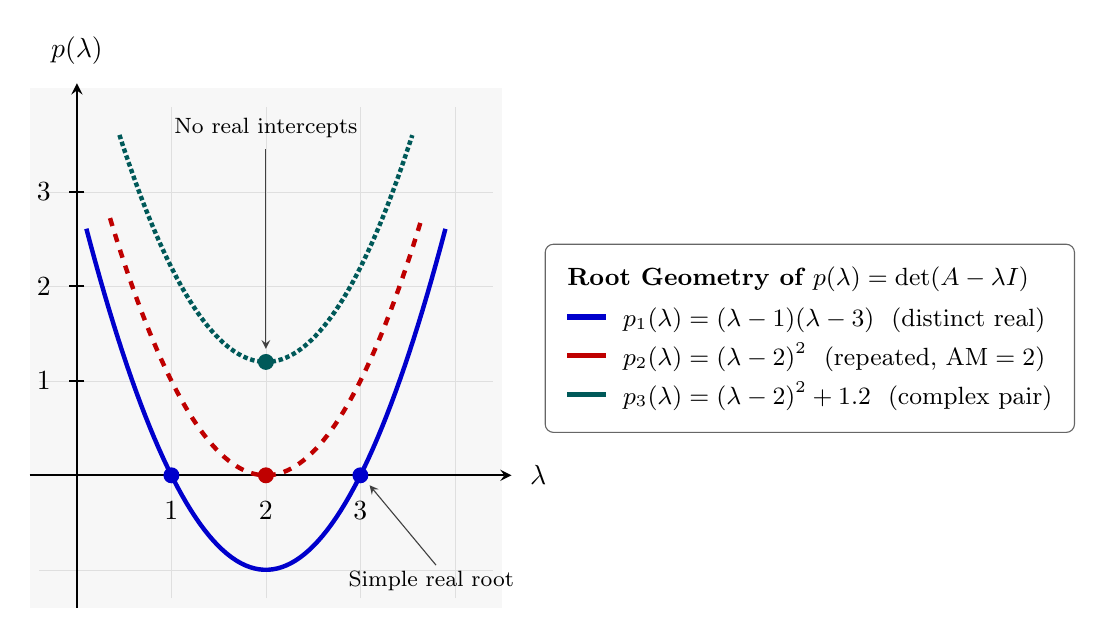
\begin{tikzpicture}[scale=1.2]
% Layer 1: Background fill
\fill[gray!6] (-0.5,-1.4) rectangle (4.5,4.1);

% Layer 2: Grid and Axes
\draw[gray!25, very thin] (-0.4,-1.3) grid (4.4,3.9);
\draw[->, >=stealth, thick] (-0.5,0) -- (4.6,0) node[right=3pt, black] {$\lambda$};
\draw[->, >=stealth, thick] (0,-1.4) -- (0,4.15) node[above=3pt, black] {$p(\lambda)$};

% Microscopic tick marks
\draw[thick] (1,0.08) -- (1,-0.08) node[below=3pt, black] {$1$};
\draw[thick] (2,0.08) -- (2,-0.08) node[below=3pt, black] {$2$};
\draw[thick] (3,0.08) -- (3,-0.08) node[below=3pt, black] {$3$};
\draw[thick] (0.08,1) -- (-0.08,1) node[left=3pt, black] {$1$};
\draw[thick] (0.08,2) -- (-0.08,2) node[left=3pt, black] {$2$};
\draw[thick] (0.08,3) -- (-0.08,3) node[left=3pt, black] {$3$};

% Layer 3: Primary Curves and Root Markers
\draw[blue!80!black, ultra thick, domain=0.1:3.9, samples=80] plot (\x, {(\x-1)*(\x-3)});
\draw[red!75!black, ultra thick, dashed, domain=0.35:3.65, samples=80] plot (\x, {(\x-2)^2});
\draw[teal!70!black, ultra thick, densely dotted, domain=0.45:3.55, samples=80] plot (\x, {(\x-2)^2 + 1.2});

\fill[blue!80!black] (1,0) circle (2.4pt);
\fill[blue!80!black] (3,0) circle (2.4pt);
\fill[red!75!black] (2,0) circle (2.4pt);
\fill[teal!70!black] (2,1.2) circle (2.4pt);

% Off-axis callouts
\draw[->, >=stealth, shorten >=2pt, black!75] (3.8,-0.95) -- (3.06,-0.06);
\draw[->, >=stealth, shorten >=2pt, black!75] (2.0,3.45) -- (2.0,1.28);

% Layer 4: Labels and Single-Node Legend
\node[black, font=\footnotesize, align=center] at (3.75,-1.12) {Simple real root};
\node[black, font=\footnotesize, align=center] at (2.0,3.68) {No real intercepts};

\node[draw=black!60, fill=white, rounded corners=3pt, align=left, inner sep=8pt, anchor=west, text=black, font=\small] at (4.95,1.45) {
\textbf{Root Geometry of $p(\lambda) = \det(A - \lambda I)$}\\[4pt]
\textcolor{blue!80!black}{\rule[2.5pt]{14pt}{2pt}}\ \ $\displaystyle p_1(\lambda) = (\lambda - 1)(\lambda - 3)$ \ (distinct real)\\[3pt]
\textcolor{red!75!black}{\rule[2.5pt]{14pt}{2pt}}\ \ $\displaystyle p_2(\lambda) = (\lambda - 2)^2$ \ (repeated, $\operatorname{AM}=2$)\\[3pt]
\textcolor{teal!70!black}{\rule[2.5pt]{14pt}{2pt}}\ \ $\displaystyle p_3(\lambda) = (\lambda - 2)^2 + 1.2$ \ (complex pair)
};
\end{tikzpicture}
\caption{Visualizing how the roots of a quadratic characteristic polynomial correspond to distinct real eigenvalues, repeated eigenvalues (tangency), and complex conjugate eigenvalues.}
\end{figure}

\newpage

\section{Problem Sets}

\subsection{Foundational Computations and Multiplicity (Problems 1--5)}

\noindent\textbf{Problem 1.} Find the characteristic polynomial $p(\lambda) = \det(A - \lambda I)$ and all eigenvalues of the symmetric matrix
\[
A = \begin{bmatrix} 4 & 6 \\ 6 & 4 \end{bmatrix}.
\]

\noindent\textbf{Problem 2.} Using both direct determinant expansion of $(B - \lambda I)$ and the $2 \times 2$ trace-determinant shortcut formula, find the characteristic polynomial and all eigenvalues of
\[
B = \begin{bmatrix} -3 & 5 \\ 2 & 0 \end{bmatrix}.
\]

\noindent\textbf{Problem 3.} Find the characteristic polynomial, all eigenvalues, and their algebraic multiplicities for the matrix
\[
A = \begin{bmatrix} 9 & -4 \\ 4 & 1 \end{bmatrix}.
\]

\noindent\textbf{Problem 4.} Determine all real values of the parameter $k$ such that the matrix
\[
A_k = \begin{bmatrix} 6 & k \\ -2 & 2 \end{bmatrix}
\]
has a single repeated eigenvalue of algebraic multiplicity $2$. For each such value of $k$, find the repeated eigenvalue.

\noindent\textbf{Problem 5.} Find the characteristic polynomial (in both factored and fully expanded forms) and list all eigenvalues with their algebraic multiplicities for the $3 \times 3$ matrix
\[
C = \begin{bmatrix} 4 & 1 & 0 \\ -1 & 2 & 0 \\ 3 & 5 & 3 \end{bmatrix}.
\]

\subsection{Strategic Expansions and Triangular Matrices (Problems 6--11)}

\noindent\textbf{Problem 6.} Using an advantageous cofactor expansion along a row or column containing a zero, find the characteristic polynomial $p(\lambda) = \det(A - \lambda I)$ of
\[
A = \begin{bmatrix} 2 & 0 & -1 \\ 1 & 4 & -1 \\ 0 & 5 & 0 \end{bmatrix}.
\]

\noindent\textbf{Problem 7.} Find the characteristic polynomial (in both pre-factored and fully expanded forms) and all eigenvalues of
\[
A = \begin{bmatrix} 8 & 4 & 3 \\ 0 & -1 & 0 \\ 2 & 5 & 7 \end{bmatrix}.
\]

\noindent\textbf{Problem 8.} Find the characteristic polynomial and all eigenvalues (with algebraic multiplicities) of the matrix
\[
A = \begin{bmatrix} 3 & 1 & -1 \\ 2 & 2 & -1 \\ 2 & 2 & 0 \end{bmatrix}.
\]
\textit{Hint:} After expanding $\det(A - \lambda I)$, apply the Rational Root Theorem to factor the resulting cubic polynomial.

\noindent\textbf{Problem 9.} Without blindly multiplying out all cubic terms first, compute $\det(A - \lambda I)$ for the dense matrix
\[
A = \begin{bmatrix} 2 & 1 & 1 \\ 1 & 2 & 1 \\ 1 & 1 & 2 \end{bmatrix}
\]
by factoring out a common linear factor during cofactor expansion. State both the factored and expanded forms of $p(\lambda)$ and all eigenvalues with their algebraic multiplicities.

\noindent\textbf{Problem 10.} Find the characteristic polynomial and list all eigenvalues, repeated according to their algebraic multiplicities, of the $4 \times 4$ lower triangular matrix
\[
A = \begin{bmatrix}
-2 & 0 & 0 & 0 \\
8 & 4 & 0 & 0 \\
-3 & 5 & -2 & 0 \\
9 & -1 & 7 & 4
\end{bmatrix}.
\]

\noindent\textbf{Problem 11.} Find the characteristic polynomial and all eigenvalues (with algebraic multiplicities) of the $4 \times 4$ block upper-triangular matrix
\[
M = \begin{bmatrix}
3 & 2 & 7 & -1 \\
1 & 4 & 0 & 5 \\
0 & 0 & 6 & -3 \\
0 & 0 & 2 & 1
\end{bmatrix}.
\]

\subsection{Trace, Determinant, and Conceptual Properties (Problems 12--17)}

\noindent\textbf{Problem 12.} Suppose the $2 \times 2$ matrix
\[
A = \begin{bmatrix} a & 3 \\ -2 & b \end{bmatrix}
\]
has eigenvalues $\lambda_1 = 4$ and $\lambda_2 = -1$. Without expanding $\det(A - \lambda I)$ directly, use the trace and determinant properties of eigenvalues to find all possible ordered pairs $(a, b)$.

\noindent\textbf{Problem 13.} Let $A$ be an $n \times n$ matrix whose characteristic polynomial factors as
\[
p(\lambda) = \det(A - \lambda I) = (\lambda_1 - \lambda)(\lambda_2 - \lambda)\cdots(\lambda_n - \lambda).
\]
\begin{enumerate}[label=(\alph*), topsep=3pt, itemsep=3pt]
    \item Prove that $\det(A - cI) = \prod_{i=1}^{n} (\lambda_i - c)$ for any scalar $c$, and deduce that $\det(A) = \prod_{i=1}^{n} \lambda_i$.
    \item For the case $n = 3$, prove that $\operatorname{tr}(A) = \lambda_1 + \lambda_2 + \lambda_3$ by comparing the $\lambda^2$ coefficient in the cofactor expansion of $\det(A - \lambda I)$ with that of $(\lambda_1 - \lambda)(\lambda_2 - \lambda)(\lambda_3 - \lambda)$.
\end{enumerate}

\noindent\textbf{Problem 14.} A $4 \times 4$ matrix $A$ has characteristic polynomial
\[
p(\lambda) = \det(A - \lambda I) = \lambda^4 - 7\lambda^3 + 11\lambda^2 + 7\lambda - 12.
\]
Without knowing the entries of $A$, determine:
\begin{enumerate}[label=(\alph*), topsep=3pt, itemsep=3pt]
    \item $\operatorname{tr}(A)$ and $\det(A)$;
    \item $\det(A - 2I)$ and $\det(A + I)$;
    \item whether $A$ is invertible, and find all eigenvalues of $A$.
\end{enumerate}

\noindent\textbf{Problem 15.} Determine whether each statement is True or False. Provide a rigorous proof if True, or an explicit counterexample if False.
\begin{enumerate}[label=(\alph*), topsep=3pt, itemsep=3pt]
    \item If $A$ is an $n \times n$ matrix satisfying $\operatorname{tr}(A) = 0$, then $0$ must be an eigenvalue of $A$.
    \item If $0$ is an eigenvalue of an $n \times n$ matrix $A$, then $A^2$ is not invertible.
\end{enumerate}

\noindent\textbf{Problem 16.} Answer the following conceptual questions:
\begin{enumerate}[label=(\alph*), topsep=3pt, itemsep=3pt]
    \item Suppose $A$ is a $3 \times 3$ matrix and $Ax = 4x$ for some nonzero vector $x \in \mathbb{R}^3$. Explain algebraically why $\det(A - 4I) = 0$, and describe geometrically what the linear transformation $T(v) = (A - 4I)v$ does to $\mathbb{R}^3$.
    \item \textbf{(True/False)} If $A$ and $B$ are $2 \times 2$ matrices with eigenvalues $\lambda_1, \lambda_2$ for $A$ and $\mu_1, \mu_2$ for $B$, then the eigenvalues of $A + B$ must be $\lambda_1 + \mu_1$ and $\lambda_2 + \mu_2$ (under some pairing).
\end{enumerate}

\noindent\textbf{Problem 17.} Determine whether each statement is True or False, and justify your answer rigorously:
\begin{enumerate}[label=(\alph*), topsep=3pt, itemsep=3pt]
    \item For every square matrix $A$, $A$ and its transpose $A^T$ have the exact same characteristic polynomial and eigenvalues.
    \item If $A$ is invertible and $\lambda$ is an eigenvalue of $A$, then $\lambda \neq 0$ and $\frac{1}{\lambda}$ is an eigenvalue of $A^{-1}$.
\end{enumerate}

\subsection{Similarity, Matrix Functions, and Diagonalization (Problems 18--21)}

\noindent\textbf{Problem 18.} Answer both parts concerning matrix similarity:
\begin{enumerate}[label=(\alph*), topsep=3pt, itemsep=3pt]
    \item Prove that if $C = PAP^{-1}$ for some invertible matrix $P$, then $C$ and $A$ share the exact same characteristic polynomial, trace, and determinant.
    \item Could the matrices
    \[
    M = \begin{bmatrix} 5 & 1 \\ 1 & 2 \end{bmatrix} \quad \text{and} \quad N = \begin{bmatrix} 4 & 0 \\ 0 & 3 \end{bmatrix}
    \]
    be similar? Justify your conclusion without attempting to solve for an invertible matrix $P$.
\end{enumerate}

\noindent\textbf{Problem 19.} Let $A = \begin{bmatrix} 1 & 2 \\ 3 & 2 \end{bmatrix}$.
\begin{enumerate}[label=(\alph*), topsep=3pt, itemsep=3pt]
    \item Find all eigenvalues of $A$.
    \item Prove in general that if $\lambda$ is an eigenvalue of a square matrix $M$, then $\lambda^k$ is an eigenvalue of $M^k$ for every integer $k \ge 1$, and $q(\lambda)$ is an eigenvalue of $q(M) = c_m M^m + \dots + c_1 M + c_0 I$ for any polynomial $q(t)$.
    \item Using parts (a) and (b), determine the eigenvalues and determinant of $A^3 - 2A + 5I$, and verify your determinant by computing $A^3 - 2A + 5I$ directly.
\end{enumerate}

\noindent\textbf{Problem 20.} Consider the matrix $A = \begin{bmatrix} 5 & -6 \\ 2 & -2 \end{bmatrix}$.
\begin{enumerate}[label=(\alph*), topsep=3pt, itemsep=3pt]
    \item Find the characteristic polynomial and eigenvalues of $A$.
    \item Find an eigenvector for each eigenvalue, and factor $A$ as $A = PDP^{-1}$ where $D$ is diagonal.
    \item Use $A^k = PD^kP^{-1}$ to derive a closed-form formula for $A^k$ (for any integer $k \ge 1$), and evaluate $A^4$.
\end{enumerate}

\noindent\textbf{Problem 21.} Let $A$ and $B$ be $n \times n$ matrices.
\begin{enumerate}[label=(\alph*), topsep=3pt, itemsep=3pt]
    \item Assuming $A$ is invertible, prove that $AB$ and $BA$ have the exact same characteristic polynomial and eigenvalues.
    \item Verify directly that even when neither $A$ nor $B$ is invertible, $AB$ and $BA$ can still share the exact same characteristic polynomial by testing
    \[
    A = \begin{bmatrix} 1 & 2 \\ 0 & 0 \end{bmatrix} \quad \text{and} \quad B = \begin{bmatrix} 1 & 0 \\ 2 & 0 \end{bmatrix}.
    \]
\end{enumerate}

\subsection{Complex Eigenvalues and Defective Matrices (Problems 22--27)}

\noindent\textbf{Problem 22.} Consider the 2D rotation-scaling matrix
\[
A = \begin{bmatrix} 3 & -4 \\ 4 & 3 \end{bmatrix}.
\]
\begin{enumerate}[label=(\alph*), topsep=3pt, itemsep=3pt]
    \item Find the characteristic polynomial and all complex eigenvalues of $A$.
    \item Express $A$ in the form $r \begin{bmatrix} \cos\theta & -\sin\theta \\ \sin\theta & \cos\theta \end{bmatrix}$, state the scaling factor $r = |\lambda|$ and counterclockwise rotation angle $\theta$, and explain geometrically why $A$ has no real eigenvalues.
\end{enumerate}

\noindent\textbf{Problem 23.} Find the characteristic polynomial, all complex eigenvalues, and one corresponding complex eigenvector for each eigenvalue of the matrix
\[
A = \begin{bmatrix} 1 & -5 \\ 2 & -1 \end{bmatrix}.
\]

\noindent\textbf{Problem 24.} Find the characteristic polynomial (in factored and expanded forms) and all real and complex eigenvalues of the $3 \times 3$ matrix
\[
A = \begin{bmatrix} 2 & 0 & 0 \\ 3 & -2 & -5 \\ 1 & 1 & 2 \end{bmatrix}.
\]

\noindent\textbf{Problem 25.} Consider the matrix
\[
A = \begin{bmatrix} 5 & 2 & 0 \\ 0 & 5 & 0 \\ -1 & 3 & 2 \end{bmatrix}.
\]
Find all eigenvalues of $A$, determine the algebraic multiplicity and geometric multiplicity of each eigenvalue by finding a basis for each eigenspace, and state whether $A$ is defective or diagonalizable.

\noindent\textbf{Problem 26.} Consider the two $3 \times 3$ matrices
\[
A = \begin{bmatrix} 2 & 0 & 1 \\ 1 & 1 & -1 \\ 0 & 0 & 2 \end{bmatrix} \quad \text{and} \quad B = \begin{bmatrix} 2 & 0 & 0 \\ 1 & 1 & -1 \\ 0 & 0 & 2 \end{bmatrix}.
\]
\begin{enumerate}[label=(\alph*), topsep=3pt, itemsep=3pt]
    \item Show that $A$ and $B$ have the exact same characteristic polynomial and eigenvalues.
    \item For the repeated eigenvalue $\lambda = 2$, compute the geometric multiplicity of $\lambda = 2$ in $A$ and in $B$. Which matrix is defective, which is diagonalizable, and can $A$ and $B$ be similar?
\end{enumerate}

\noindent\textbf{Problem 27.} Consider the parameterized matrix
\[
A_c = \begin{bmatrix} 3 & c & 1 \\ 0 & 3 & 0 \\ 0 & 2 & -1 \end{bmatrix}, \quad c \in \mathbb{R}.
\]
\begin{enumerate}[label=(\alph*), topsep=3pt, itemsep=3pt]
    \item Find the characteristic polynomial and eigenvalues of $A_c$, noting whether they depend on $c$.
    \item Find the algebraic and geometric multiplicities of each eigenvalue as a function of $c$. For which value(s) of $c$ is $A_c$ diagonalizable (non-defective), and for which value(s) is it defective?
\end{enumerate}

\subsection{Real-World Modeling: PCA and Markov Chains (Problems 28--30)}

\noindent\textbf{Problem 28.} In quantitative finance, the sample covariance matrix of daily returns (in $\%^2$) for two correlated technology equities is
\[
\Sigma = \begin{bmatrix} 5 & 2 \\ 2 & 2 \end{bmatrix}.
\]
\begin{enumerate}[label=(\alph*), topsep=3pt, itemsep=3pt]
    \item Find the characteristic polynomial and eigenvalues $\lambda_1 \ge \lambda_2$ of $\Sigma$, verifying that both are real and non-negative.
    \item Compute the total variance $\operatorname{tr}(\Sigma)$ and determine the exact fraction (and percentage) of total variance explained by the first principal component.
    \item Find a unit eigenvector $v_1$ corresponding to $\lambda_1$ (the first principal component loading vector).
\end{enumerate}

\noindent\textbf{Problem 29.} An algorithmic trading model uses a $3$-factor centered covariance matrix
\[
\Sigma = \begin{bmatrix} 6 & 0 & 4 \\ 0 & 4 & 0 \\ 4 & 0 & 6 \end{bmatrix}.
\]
\begin{enumerate}[label=(\alph*), topsep=3pt, itemsep=3pt]
    \item Find all eigenvalues $\lambda_1 \ge \lambda_2 \ge \lambda_3$ of $\Sigma$ by strategically expanding $\det(\Sigma - \lambda I) = 0$.
    \item Verify your eigenvalues using $\operatorname{tr}(\Sigma)$ and $\det(\Sigma)$.
    \item If the model projects the feature space onto the top $k$ principal components needed to capture at least $80\%$ of total variance, find the minimum required dimension $k$ and the exact percentage of variance captured.
\end{enumerate}

\noindent\textbf{Problem 30.} A quantitative analyst models daily transitions between two market regimes—Bull (State $1$) and Bear (State $2$)—using the column-stochastic transition matrix
\[
T = \begin{bmatrix} 0.8 & 0.3 \\ 0.2 & 0.7 \end{bmatrix},
\]
where $T_{ij}$ denotes the probability of moving from regime $j$ today to regime $i$ tomorrow.
\begin{enumerate}[label=(\alph*), topsep=3pt, itemsep=3pt]
    \item Find the characteristic polynomial and all eigenvalues of $T$, and explain why $\lambda = 1$ must be an eigenvalue of any column-stochastic matrix.
    \item Find the steady-state probability vector $\pi = \begin{bmatrix} \pi_1 \\ \pi_2 \end{bmatrix}$ (an eigenvector for $\lambda = 1$ with non-negative entries summing to $1$).
    \item Express the initial state $x_0 = \begin{bmatrix} 1 \\ 0 \end{bmatrix}$ as a linear combination of eigenvectors of $T$, and evaluate $\lim_{k \to \infty} T^k x_0$.
\end{enumerate}

\subsection{Diagnostic Testing: Find the Flaw (Problems 31--34)}

\noindent\textbf{Problem 31.} \textit{Find the Flaw:} Below is a student's attempt to find the characteristic polynomial and eigenvalues of $A = \begin{bmatrix} 5 & 4 \\ 1 & 2 \end{bmatrix}$:
\begin{quote}
\textbf{Flawed Solution:} Using the $2 \times 2$ shortcut formula, the characteristic polynomial is $p(\lambda) = \lambda^2 + \operatorname{tr}(A)\lambda + \det(A)$. Here $\operatorname{tr}(A) = 5 + 2 = 7$ and $\det(A) = (5)(2) - (4)(1) = 6$. Therefore, $p(\lambda) = \lambda^2 + 7\lambda + 6 = (\lambda + 6)(\lambda + 1) = 0$, yielding eigenvalues $\lambda_1 = -6$ and $\lambda_2 = -1$.
\end{quote}
Identify the flaw, explain why it is wrong in one clear sentence, and provide the correct characteristic polynomial and eigenvalues.

\noindent\textbf{Problem 32.} \textit{Find the Flaw:} Below is a student's attempt to find the characteristic polynomial and eigenvalues of $A = \begin{bmatrix} 2 & -1 & 4 \\ 0 & 5 & 3 \\ 0 & 0 & -3 \end{bmatrix}$:
\begin{quote}
\textbf{Flawed Solution:} Setting up $\det(A - \lambda I) = 0$ and expanding along the first column gives
\[
\det\begin{bmatrix} 2 - \lambda & -1 & 4 \\ 0 & 5 & 3 \\ 0 & 0 & -3 \end{bmatrix} = (2 - \lambda)\big[(5)(-3) - (3)(0)\big] = (2 - \lambda)(-15) = 15\lambda - 30.
\]
Setting $15\lambda - 30 = 0$, the only eigenvalue is $\lambda = 2$.
\end{quote}
Identify the flaw, explain why it is wrong in one clear sentence, and provide the correct characteristic polynomial (factored and expanded) and all eigenvalues.

\noindent\textbf{Problem 33.} \textit{Find the Flaw:} Below is a student's attempt to find the eigenvalues of $A^3$ for $A = \begin{bmatrix} 2 & 3 \\ 1 & 4 \end{bmatrix}$:
\begin{quote}
\textbf{Flawed Solution:} First we find the eigenvalues of $A$: $\operatorname{tr}(A) = 6$ and $\det(A) = 8 - 3 = 5$, so $p(\lambda) = \lambda^2 - 6\lambda + 5 = (\lambda - 5)(\lambda - 1) = 0$. Thus $A$ has eigenvalues $5$ and $1$. To find the eigenvalues of $A^3$, we multiply each eigenvalue of $A$ by $3$, giving eigenvalues $15$ and $3$.
\end{quote}
Identify the flaw, explain why it is wrong in one clear sentence, and provide the correct eigenvalues of $A^3$ (along with a trace/determinant verification).

\noindent\textbf{Problem 34.} \textit{Find the Flaw:} Below is a student's attempt to determine whether a $3 \times 3$ matrix $A$ with characteristic polynomial $p(\lambda) = -\lambda^3 + 8\lambda^2 - 16\lambda$ is invertible:
\begin{quote}
\textbf{Flawed Solution:} Factoring gives $p(\lambda) = -\lambda(\lambda^2 - 8\lambda + 16) = -\lambda(\lambda - 4)^2$. The roots are $\lambda = 0$ and $\lambda = 4$. Because $\lambda = 4$ is a nonzero eigenvalue with algebraic multiplicity $2$ (accounting for the majority of the eigenvalues), the matrix stretches vectors along those directions, so $A$ is invertible.
\end{quote}
Identify the flaw, explain why it is wrong in one clear sentence, and provide the correct conclusion supported by $\det(A)$ and the Invertible Matrix Theorem.

\newpage

\section{Detailed Solutions}

\subsection{Solutions to Foundational Computations and Multiplicity (Problems 1--5)}

\noindent\textbf{Problem 1}

\textbf{Original Problem:} Find the characteristic polynomial $p(\lambda) = \det(A - \lambda I)$ and all eigenvalues of the symmetric matrix $A = \begin{bmatrix} 4 & 6 \\ 6 & 4 \end{bmatrix}$.

\textbf{Solution:} First, subtract $\lambda I$ from $A$:
\[
A - \lambda I = \begin{bmatrix} 4 - \lambda & 6 \\ 6 & 4 - \lambda \end{bmatrix}.
\]
Compute the determinant to obtain the characteristic polynomial:
\begin{align*}
p(\lambda) = \det(A - \lambda I) &= (4 - \lambda)(4 - \lambda) - (6)(6) \\
&= (16 - 8\lambda + \lambda^2) - 36 \\
&= \lambda^2 - 8\lambda - 20.
\end{align*}
Setting $p(\lambda) = 0$ and factoring yields:
\[
\lambda^2 - 8\lambda - 20 = (\lambda - 10)(\lambda + 2) = 0 \implies \lambda_1 = 10, \quad \lambda_2 = -2.
\]
\textit{Verification:} $\lambda_1 + \lambda_2 = 10 + (-2) = 8 = \operatorname{tr}(A)$ and $\lambda_1 \lambda_2 = (10)(-2) = -20 = 16 - 36 = \det(A)$.

\noindent\rule{\textwidth}{0.4pt}

\noindent\textbf{Problem 2}

\textbf{Original Problem:} Using both direct determinant expansion of $(B - \lambda I)$ and the $2 \times 2$ trace-determinant shortcut formula, find the characteristic polynomial and all eigenvalues of $B = \begin{bmatrix} -3 & 5 \\ 2 & 0 \end{bmatrix}$.

\textbf{Solution:}
\textit{Method 1 (Direct Determinant):}
\[
B - \lambda I = \begin{bmatrix} -3 - \lambda & 5 \\ 2 & -\lambda \end{bmatrix},
\]
so
\[
p(\lambda) = \det(B - \lambda I) = (-3 - \lambda)(-\lambda) - (5)(2) = \lambda^2 + 3\lambda - 10.
\]
\textit{Method 2 (Trace-Determinant Shortcut):}
We compute $\operatorname{tr}(B) = -3 + 0 = -3$ and $\det(B) = (-3)(0) - (5)(2) = -10$. Substituting into $\lambda^2 - \operatorname{tr}(B)\lambda + \det(B)$ gives
\[
p(\lambda) = \lambda^2 - (-3)\lambda + (-10) = \lambda^2 + 3\lambda - 10.
\]
Both methods agree. Setting $p(\lambda) = 0$ and factoring:
\[
\lambda^2 + 3\lambda - 10 = (\lambda + 5)(\lambda - 2) = 0 \implies \lambda_1 = -5, \quad \lambda_2 = 2.
\]

\noindent\rule{\textwidth}{0.4pt}

\noindent\textbf{Problem 3}

\textbf{Original Problem:} Find the characteristic polynomial, all eigenvalues, and their algebraic multiplicities for the matrix $A = \begin{bmatrix} 9 & -4 \\ 4 & 1 \end{bmatrix}$.

\textbf{Solution:} Form $(A - \lambda I)$:
\[
A - \lambda I = \begin{bmatrix} 9 - \lambda & -4 \\ 4 & 1 - \lambda \end{bmatrix}.
\]
Compute the determinant:
\begin{align*}
p(\lambda) = \det(A - \lambda I) &= (9 - \lambda)(1 - \lambda) - (-4)(4) \\
&= (9 - 10\lambda + \lambda^2) + 16 \\
&= \lambda^2 - 10\lambda + 25.
\end{align*}
Factoring the quadratic as a perfect square:
\[
\lambda^2 - 10\lambda + 25 = (\lambda - 5)^2 = 0.
\]
\textit{Verification:} $\operatorname{tr}(A) = 9 + 1 = 10 = 5 + 5$ and $\det(A) = 9 + 16 = 25 = 5 \cdot 5$.
Thus, the characteristic polynomial is $\lambda^2 - 10\lambda + 25 = (\lambda - 5)^2$, and the sole eigenvalue is $\lambda = 5$ with algebraic multiplicity $2$.

\noindent\rule{\textwidth}{0.4pt}

\noindent\textbf{Problem 4}

\textbf{Original Problem:} Determine all real values of the parameter $k$ such that the matrix $A_k = \begin{bmatrix} 6 & k \\ -2 & 2 \end{bmatrix}$ has a single repeated eigenvalue of algebraic multiplicity $2$. For each such value of $k$, find the repeated eigenvalue.

\textbf{Solution:} Compute $\operatorname{tr}(A_k) = 6 + 2 = 8$ and $\det(A_k) = (6)(2) - (k)(-2) = 12 + 2k$. Using the $2 \times 2$ shortcut formula, the characteristic polynomial is
\[
p(\lambda) = \lambda^2 - 8\lambda + (12 + 2k).
\]
A quadratic polynomial $a\lambda^2 + b\lambda + c$ has a repeated root of algebraic multiplicity $2$ if and only if its discriminant $\Delta = b^2 - 4ac$ equals $0$:
\[
\Delta = (-8)^2 - 4(1)(12 + 2k) = 64 - 48 - 8k = 16 - 8k = 0 \implies k = 2.
\] When $k = 2$, the matrix is
\[
A_2 = \begin{bmatrix} 6 & 2 \\ -2 & 2 \end{bmatrix}, \qquad p(\lambda) = \lambda^2 - 8\lambda + 16 = (\lambda - 4)^2 = 0.
\]
\textit{Verification:} Direct calculation gives $\det(A_2 - \lambda I) = (6 - \lambda)(2 - \lambda) + 4 = (\lambda - 4)^2$. Thus, $k = 2$ is the unique value, producing the repeated eigenvalue $\lambda = 4$ with algebraic multiplicity $2$.

\noindent\rule{\textwidth}{0.4pt}

\noindent\textbf{Problem 5}

\textbf{Original Problem:} Find the characteristic polynomial (in both factored and fully expanded forms) and list all eigenvalues with their algebraic multiplicities for the $3 \times 3$ matrix $C = \begin{bmatrix} 4 & 1 & 0 \\ -1 & 2 & 0 \\ 3 & 5 & 3 \end{bmatrix}$.

\textbf{Solution:} Set up $(C - \lambda I)$ and expand the determinant down the third column (which contains two zeros):
\begin{align*}
p(\lambda) = \det(C - \lambda I) &= \det\begin{bmatrix} 4 - \lambda & 1 & 0 \\ -1 & 2 - \lambda & 0 \\ 3 & 5 & 3 - \lambda \end{bmatrix} \\
&= (3 - \lambda)\det\begin{bmatrix} 4 - \lambda & 1 \\ -1 & 2 - \lambda \end{bmatrix} \\
&= (3 - \lambda)\big[(4 - \lambda)(2 - \lambda) - (-1)(1)\big] \\
&= (3 - \lambda)(\lambda^2 - 6\lambda + 9) \\
&= (3 - \lambda)(\lambda - 3)^2 = (3 - \lambda)^3 = -(\lambda - 3)^3.
\end{align*}
Expanding completely:
\[
p(\lambda) = (3 - \lambda)(\lambda^2 - 6\lambda + 9) = -\lambda^3 + 9\lambda^2 - 27\lambda + 27.
\]
\textit{Verification:} $\operatorname{tr}(C) = 4 + 2 + 3 = 9 = 3 + 3 + 3$, and $\det(C) = p(0) = 27 = 3^3$.
Hence, the sole eigenvalue is $\lambda = 3$ with algebraic multiplicity $3$.

\subsection{Solutions to Strategic Expansions and Triangular Matrices (Problems 6--11)}

\noindent\textbf{Problem 6}

\textbf{Original Problem:} Using an advantageous cofactor expansion along a row or column containing a zero, find the characteristic polynomial $p(\lambda) = \det(A - \lambda I)$ of $A = \begin{bmatrix} 2 & 0 & -1 \\ 1 & 4 & -1 \\ 0 & 5 & 0 \end{bmatrix}$.

\textbf{Solution:} Form $(A - \lambda I)$:
\[
A - \lambda I = \begin{bmatrix} 2 - \lambda & 0 & -1 \\ 1 & 4 - \lambda & -1 \\ 0 & 5 & -\lambda \end{bmatrix}.
\]
Expanding along the first row (cofactor signs $+, -, +$) leverages the zero in entry $(1, 2)$:
\begin{align*}
p(\lambda) = \det(A - \lambda I) &= (2 - \lambda)\det\begin{bmatrix} 4 - \lambda & -1 \\ 5 & -\lambda \end{bmatrix} - 0 + (-1)\det\begin{bmatrix} 1 & 4 - \lambda \\ 0 & 5 \end{bmatrix} \\
&= (2 - \lambda)\big[(4 - \lambda)(-\lambda) - (-5)\big] - 1\big[(1)(5) - 0\big] \\
&= (2 - \lambda)(\lambda^2 - 4\lambda + 5) - 5 \\
&= (2\lambda^2 - 8\lambda + 10 - \lambda^3 + 4\lambda^2 - 5\lambda) - 5 \\
&= -\lambda^3 + 6\lambda^2 - 13\lambda + 5.
\end{align*}
\textit{Verification:} The coefficient of $\lambda^2$ is $6 = \operatorname{tr}(A) = 2 + 4 + 0$, and $p(0) = 5 = 2(0 + 5) - 1(5 - 0) = \det(A)$.

\noindent\rule{\textwidth}{0.4pt}

\noindent\textbf{Problem 7}

\textbf{Original Problem:} Find the characteristic polynomial (in both pre-factored and fully expanded forms) and all eigenvalues of $A = \begin{bmatrix} 8 & 4 & 3 \\ 0 & -1 & 0 \\ 2 & 5 & 7 \end{bmatrix}$.

\textbf{Solution:} Form $(A - \lambda I)$ and expand along the second row, which has two zeros (cofactor signs $-, +, -$):
\begin{align*}
p(\lambda) = \det(A - \lambda I) &= \det\begin{bmatrix} 8 - \lambda & 4 & 3 \\ 0 & -1 - \lambda & 0 \\ 2 & 5 & 7 - \lambda \end{bmatrix} \\
&= -0 + (-1 - \lambda)\det\begin{bmatrix} 8 - \lambda & 3 \\ 2 & 7 - \lambda \end{bmatrix} - 0 \\
&= -(\lambda + 1)\big[(8 - \lambda)(7 - \lambda) - (3)(2)\big] \\
&= -(\lambda + 1)(\lambda^2 - 15\lambda + 56 - 6) \\
&= -(\lambda + 1)(\lambda^2 - 15\lambda + 50) \\
&= -(\lambda + 1)(\lambda - 5)(\lambda - 10).
\end{align*}
Expanding fully gives:
\[
p(\lambda) = -(\lambda^3 - 15\lambda^2 + 50\lambda + \lambda^2 - 15\lambda + 50) = -\lambda^3 + 14\lambda^2 - 35\lambda - 50.
\]
\textit{Verification:} $\operatorname{tr}(A) = 8 + (-1) + 7 = 14 = -1 + 5 + 10$, and $\det(A) = (-1)(56 - 6) = -50 = (-1)(5)(10) = p(0)$.
The eigenvalues are $\lambda_1 = -1$, $\lambda_2 = 5$, and $\lambda_3 = 10$ (each with algebraic multiplicity $1$).

\noindent\rule{\textwidth}{0.4pt}

\noindent\textbf{Problem 8}

\textbf{Original Problem:} Find the characteristic polynomial and all eigenvalues (with algebraic multiplicities) of the matrix $A = \begin{bmatrix} 3 & 1 & -1 \\ 2 & 2 & -1 \\ 2 & 2 & 0 \end{bmatrix}$. \textit{Hint:} After expanding $\det(A - \lambda I)$, apply the Rational Root Theorem to factor the resulting cubic polynomial.

\textbf{Solution:} Form $(A - \lambda I)$ and expand down the third column (or along the third row) to utilize the zero in entry $(3, 3)$:
\begin{align*}
p(\lambda) = \det(A - \lambda I) &= \det\begin{bmatrix} 3 - \lambda & 1 & -1 \\ 2 & 2 - \lambda & -1 \\ 2 & 2 & -\lambda \end{bmatrix} \\
&= (-1)\det\begin{bmatrix} 2 & 2 - \lambda \\ 2 & 2 \end{bmatrix} - (-1)\det\begin{bmatrix} 3 - \lambda & 1 \\ 2 & 2 \end{bmatrix} + (-\lambda)\det\begin{bmatrix} 3 - \lambda & 1 \\ 2 & 2 - \lambda \end{bmatrix} \\
&= -1\big[4 - 2(2 - \lambda)\big] + 1\big[2(3 - \lambda) - 2\big] - \lambda\big[(3 - \lambda)(2 - \lambda) - 2\big] \\
&= -1(2\lambda) + (4 - 2\lambda) - \lambda(\lambda^2 - 5\lambda + 4) \\
&= -4\lambda + 4 - \lambda^3 + 5\lambda^2 - 4\lambda \\
&= -\lambda^3 + 5\lambda^2 - 8\lambda + 4.
\end{align*}
To find the eigenvalues, solve $\lambda^3 - 5\lambda^2 + 8\lambda - 4 = 0$. By the Rational Root Theorem, possible integer roots are divisors of $4$: $\pm 1, \pm 2, \pm 4$. Testing $\lambda = 1$ gives $1 - 5 + 8 - 4 = 0$, so $(\lambda - 1)$ is a factor. Dividing by $(\lambda - 1)$ yields:
\[
\lambda^3 - 5\lambda^2 + 8\lambda - 4 = (\lambda - 1)(\lambda^2 - 4\lambda + 4) = (\lambda - 1)(\lambda - 2)^2.
\]
Hence, $p(\lambda) = -\lambda^3 + 5\lambda^2 - 8\lambda + 4 = -(\lambda - 1)(\lambda - 2)^2$.
\textit{Verification:} $\operatorname{tr}(A) = 3 + 2 + 0 = 5 = 1 + 2 + 2$, and $\det(A) = p(0) = 4 = 1 \cdot 2 \cdot 2$.
The eigenvalues are $\lambda = 1$ (algebraic multiplicity $1$) and $\lambda = 2$ (algebraic multiplicity $2$).

\noindent\rule{\textwidth}{0.4pt}

\noindent\textbf{Problem 9}

\textbf{Original Problem:} Without blindly multiplying out all cubic terms first, compute $\det(A - \lambda I)$ for the dense matrix $A = \begin{bmatrix} 2 & 1 & 1 \\ 1 & 2 & 1 \\ 1 & 1 & 2 \end{bmatrix}$ by factoring out a common linear factor during cofactor expansion. State both the factored and expanded forms of $p(\lambda)$ and all eigenvalues with their algebraic multiplicities.

\textbf{Solution:} Expand $\det(A - \lambda I)$ along the first row while keeping linear factors unexpanded:
\begin{align*}
p(\lambda) &= \det\begin{bmatrix} 2 - \lambda & 1 & 1 \\ 1 & 2 - \lambda & 1 \\ 1 & 1 & 2 - \lambda \end{bmatrix} \\
&= (2 - \lambda)\big[(2 - \lambda)^2 - 1\big] - 1\big[(2 - \lambda) - 1\big] + 1\big[1 - (2 - \lambda)\big] \\
&= (2 - \lambda)(1 - \lambda)(3 - \lambda) - (1 - \lambda) + (\lambda - 1) \\
&= (2 - \lambda)(1 - \lambda)(3 - \lambda) - 2(1 - \lambda).
\end{align*}
Factoring out the common factor $(1 - \lambda)$ immediately avoids cubic guesswork:
\begin{align*}
p(\lambda) &= (1 - \lambda)\big[(2 - \lambda)(3 - \lambda) - 2\big] \\
&= (1 - \lambda)(\lambda^2 - 5\lambda + 6 - 2) \\
&= (1 - \lambda)(\lambda^2 - 5\lambda + 4) \\
&= (1 - \lambda)(1 - \lambda)(4 - \lambda) = (1 - \lambda)^2(4 - \lambda).
\end{align*}
Expanding fully gives:
\[
p(\lambda) = (\lambda^2 - 2\lambda + 1)(4 - \lambda) = -\lambda^3 + 6\lambda^2 - 9\lambda + 4.
\]
\textit{Verification:} $\operatorname{tr}(A) = 2 + 2 + 2 = 6 = 1 + 1 + 4$, and $\det(A) = p(0) = 4 = 1 \cdot 1 \cdot 4$.
The eigenvalues are $\lambda = 1$ (algebraic multiplicity $2$) and $\lambda = 4$ (algebraic multiplicity $1$).

\noindent\rule{\textwidth}{0.4pt}

\noindent\textbf{Problem 10}

\textbf{Original Problem:} Find the characteristic polynomial and list all eigenvalues, repeated according to their algebraic multiplicities, of the $4 \times 4$ lower triangular matrix
\[
A = \begin{bmatrix}
-2 & 0 & 0 & 0 \\
8 & 4 & 0 & 0 \\
-3 & 5 & -2 & 0 \\
9 & -1 & 7 & 4
\end{bmatrix}.
\]

\textbf{Solution:} Because $A$ is lower triangular, $(A - \lambda I)$ is also lower triangular with main diagonal entries $-2 - \lambda$, $4 - \lambda$, $-2 - \lambda$, and $4 - \lambda$. The determinant of a triangular matrix equals the product of its main diagonal entries:
\[
p(\lambda) = \det(A - \lambda I) = (-2 - \lambda)(4 - \lambda)(-2 - \lambda)(4 - \lambda) = (\lambda + 2)^2(\lambda - 4)^2.
\]
Setting $p(\lambda) = 0$ yields the eigenvalues directly: $\lambda = -2$ (algebraic multiplicity $2$) and $\lambda = 4$ (algebraic multiplicity $2$), or listed with repetitions: $-2, -2, 4, 4$.
\textit{Verification:} $\operatorname{tr}(A) = -2 + 4 - 2 + 4 = 4$, and $\det(A) = (-2)^2(4)^2 = 64 = p(0)$.

\noindent\rule{\textwidth}{0.4pt}

\noindent\textbf{Problem 11}

\textbf{Original Problem:} Find the characteristic polynomial and all eigenvalues (with algebraic multiplicities) of the $4 \times 4$ block upper-triangular matrix
\[
M = \begin{bmatrix}
3 & 2 & 7 & -1 \\
1 & 4 & 0 & 5 \\
0 & 0 & 6 & -3 \\
0 & 0 & 2 & 1
\end{bmatrix}.
\]

\textbf{Solution:} Write $M - \lambda I$ in block upper-triangular form:
\[
M - \lambda I = \begin{bmatrix} A_1 - \lambda I_2 & B \\ 0 & A_2 - \lambda I_2 \end{bmatrix}, \quad A_1 = \begin{bmatrix} 3 & 2 \\ 1 & 4 \end{bmatrix}, \quad A_2 = \begin{bmatrix} 6 & -3 \\ 2 & 1 \end{bmatrix}.
\]
Any determinant term choosing entries from the lower-left $2 \times 2$ zero block vanishes, so cofactor expansion yields $\det(M - \lambda I) = \det(A_1 - \lambda I_2)\det(A_2 - \lambda I_2)$. Computing each $2 \times 2$ characteristic polynomial via the shortcut formula:
\begin{align*}
\det(A_1 - \lambda I_2) &= \lambda^2 - (3 + 4)\lambda + (12 - 2) = \lambda^2 - 7\lambda + 10 = (\lambda - 2)(\lambda - 5), \\
\det(A_2 - \lambda I_2) &= \lambda^2 - (6 + 1)\lambda + (6 - (-6)) = \lambda^2 - 7\lambda + 12 = (\lambda - 3)(\lambda - 4).
\end{align*}
Multiplying the two polynomials gives the characteristic polynomial of $M$:
\[
p(\lambda) = (\lambda - 2)(\lambda - 3)(\lambda - 4)(\lambda - 5) = \lambda^4 - 14\lambda^3 + 71\lambda^2 - 154\lambda + 120.
\]
\textit{Verification:} $\operatorname{tr}(M) = 3 + 4 + 6 + 1 = 14 = 2 + 3 + 4 + 5$, and $\det(M) = 10 \cdot 12 = 120 = 2 \cdot 3 \cdot 4 \cdot 5 = p(0)$.
The eigenvalues are $\lambda = 2, 3, 4, 5$, each with algebraic multiplicity $1$.

\subsection{Solutions to Trace, Determinant, and Conceptual Properties (Problems 12--17)}

\noindent\textbf{Problem 12}

\textbf{Original Problem:} Suppose the $2 \times 2$ matrix $A = \begin{bmatrix} a & 3 \\ -2 & b \end{bmatrix}$ has eigenvalues $\lambda_1 = 4$ and $\lambda_2 = -1$. Without expanding $\det(A - \lambda I)$ directly, use the trace and determinant properties of eigenvalues to find all possible ordered pairs $(a, b)$.

\textbf{Solution:} Using $\operatorname{tr}(A) = \lambda_1 + \lambda_2$ and $\det(A) = \lambda_1\lambda_2$:
\begin{align*}
\operatorname{tr}(A) = a + b &= 4 + (-1) = 3 \implies b = 3 - a, \\
\det(A) = ab - (3)(-2) = ab + 6 &= (4)(-1) = -4 \implies ab = -10.
\end{align*}
Substituting $b = 3 - a$ into $ab = -10$ produces:
\[
a(3 - a) = -10 \implies a^2 - 3a - 10 = 0 \implies (a - 5)(a + 2) = 0.
\]
Thus $a = 5$ (giving $b = 3 - 5 = -2$) or $a = -2$ (giving $b = 3 - (-2) = 5$).
\textit{Verification:} For $(5, -2)$, $\operatorname{tr} = 3$ and $\det = -10 + 6 = -4$; for $(-2, 5)$, $\operatorname{tr} = 3$ and $\det = -10 + 6 = -4$; both yield $\lambda^2 - 3\lambda - 4 = (\lambda - 4)(\lambda + 1) = 0$.
The possible ordered pairs are $(a, b) = (5, -2)$ and $(a, b) = (-2, 5)$.

\noindent\rule{\textwidth}{0.4pt}

\noindent\textbf{Problem 13}

\textbf{Original Problem:} Let $A$ be an $n \times n$ matrix whose characteristic polynomial factors as $p(\lambda) = \det(A - \lambda I) = (\lambda_1 - \lambda)(\lambda_2 - \lambda)\cdots(\lambda_n - \lambda)$.
(a) Prove that $\det(A - cI) = \prod_{i=1}^{n}(\lambda_i - c)$ for any scalar $c$, and deduce that $\det(A) = \prod_{i=1}^{n}\lambda_i$.
(b) For the case $n = 3$, prove that $\operatorname{tr}(A) = \lambda_1 + \lambda_2 + \lambda_3$ by comparing the $\lambda^2$ coefficient in the cofactor expansion of $\det(A - \lambda I)$ with that of $(\lambda_1 - \lambda)(\lambda_2 - \lambda)(\lambda_3 - \lambda)$.

\textbf{Solution:}
\begin{enumerate}[label=(\alph*), topsep=3pt, itemsep=4pt]
    \item Because the polynomial identity $\det(A - \lambda I) = \prod_{i=1}^{n} (\lambda_i - \lambda)$ holds for all scalar values $\lambda$, evaluating both sides at $\lambda = c$ directly yields
    \[
    \det(A - cI) = \prod_{i=1}^{n} (\lambda_i - c).
    \]
    Setting $c = 0$ on both sides gives $\det(A - 0I) = \det(A) = \prod_{i=1}^{n} (\lambda_i - 0) = \prod_{i=1}^{n} \lambda_i$.
    \item Expanding the factored polynomial for $n = 3$ yields:
    \[
    (\lambda_1 - \lambda)(\lambda_2 - \lambda)(\lambda_3 - \lambda) = -\lambda^3 + (\lambda_1 + \lambda_2 + \lambda_3)\lambda^2 - (\lambda_1\lambda_2 + \lambda_1\lambda_3 + \lambda_2\lambda_3)\lambda + \lambda_1\lambda_2\lambda_3.
    \]
    On the other hand, expanding $\det(A - \lambda I)$ along the first row for $A = [a_{ij}]$ gives:
    \begin{align*}
    \det(A - \lambda I) &= (a_{11} - \lambda)\big[(a_{22} - \lambda)(a_{33} - \lambda) - a_{23}a_{32}\big] \\
    &\quad - a_{12}\big[a_{21}(a_{33} - \lambda) - a_{23}a_{31}\big] + a_{13}\big[a_{21}a_{32} - (a_{22} - \lambda)a_{31}\big].
    \end{align*}
    Notice that the second and third cofactor terms are at most linear in $\lambda$ (degree $\le 1$), and $-(a_{11} - \lambda)a_{23}a_{32}$ also has degree $\le 1$. Thus, every $\lambda^3$ and $\lambda^2$ term arises exclusively from the diagonal product:
    \[
    (a_{11} - \lambda)(a_{22} - \lambda)(a_{33} - \lambda) = -\lambda^3 + (a_{11} + a_{22} + a_{33})\lambda^2 + (\text{terms of degree } \le 1).
    \]
    Equating the coefficients of $\lambda^2$ in both representations of $p(\lambda)$ proves $\operatorname{tr}(A) = a_{11} + a_{22} + a_{33} = \lambda_1 + \lambda_2 + \lambda_3$.
\end{enumerate}

\noindent\rule{\textwidth}{0.4pt}

\noindent\textbf{Problem 14}

\textbf{Original Problem:} A $4 \times 4$ matrix $A$ has characteristic polynomial $p(\lambda) = \det(A - \lambda I) = \lambda^4 - 7\lambda^3 + 11\lambda^2 + 7\lambda - 12$. Without knowing the entries of $A$, determine: (a) $\operatorname{tr}(A)$ and $\det(A)$; (b) $\det(A - 2I)$ and $\det(A + I)$; (c) whether $A$ is invertible, and find all eigenvalues of $A$.

\textbf{Solution:}
\begin{enumerate}[label=(\alph*), topsep=3pt, itemsep=4pt]
    \item For a $4 \times 4$ matrix, $p(\lambda) = \prod_{i=1}^{4} (\lambda_i - \lambda) = \lambda^4 - \left(\sum_{i=1}^{4}\lambda_i\right)\lambda^3 + \dots + \prod_{i=1}^{4}\lambda_i$. Comparing coefficients, $\operatorname{tr}(A) = \sum_{i=1}^{4} \lambda_i = 7$. Evaluating at $\lambda = 0$ gives $\det(A) = p(0) = -12$.
    \item Evaluating $p(\lambda)$ at $\lambda = 2$ and $\lambda = -1$:
    \begin{align*}
    \det(A - 2I) = p(2) &= 2^4 - 7(2^3) + 11(2^2) + 7(2) - 12 = 16 - 56 + 44 + 14 - 12 = 6, \\
    \det(A + I) = \det(A - (-1)I) = p(-1) &= (-1)^4 - 7(-1)^3 + 11(-1)^2 + 7(-1) - 12 = 1 + 7 + 11 - 7 - 12 = 0.
    \end{align*}
    \item Since $\det(A) = -12 \neq 0$, $A$ is invertible. Since $p(-1) = 0$, $\lambda = -1$ is a root; testing $\lambda = 1$ gives $p(1) = 1 - 7 + 11 + 7 - 12 = 0$. Dividing by $(\lambda - 1)(\lambda + 1) = \lambda^2 - 1$ gives:
    \[
    p(\lambda) = (\lambda^2 - 1)(\lambda^2 - 7\lambda + 12) = (\lambda - 1)(\lambda + 1)(\lambda - 3)(\lambda - 4).
    \]
    The eigenvalues are $\lambda = -1, 1, 3, 4$ (all nonzero, consistent with invertibility).
\end{enumerate}

\noindent\rule{\textwidth}{0.4pt}

\noindent\textbf{Problem 15}

\textbf{Original Problem:} Determine whether each statement is True or False. Provide a rigorous proof if True, or an explicit counterexample if False. (a) If $A$ is an $n \times n$ matrix satisfying $\operatorname{tr}(A) = 0$, then $0$ must be an eigenvalue of $A$. (b) If $0$ is an eigenvalue of an $n \times n$ matrix $A$, then $A^2$ is not invertible.

\textbf{Solution:}
\begin{enumerate}[label=(\alph*), topsep=3pt, itemsep=4pt]
    \item \textbf{False.} $\operatorname{tr}(A) = \sum_{i=1}^{n}\lambda_i = 0$ only requires the sum of the eigenvalues to vanish, not any individual eigenvalue. \textit{Counterexample:} Let $A = \begin{bmatrix} 1 & 0 \\ 0 & -1 \end{bmatrix}$. Then $\operatorname{tr}(A) = 1 + (-1) = 0$, yet the eigenvalues of $A$ are $1$ and $-1$, neither of which is $0$ (indeed, $\det(A) = -1 \neq 0$).
    \item \textbf{True.} If $0$ is an eigenvalue of $A$, there exists a nonzero vector $x \neq 0$ such that $Ax = 0x = 0$. Multiplying on the left by $A$ gives
    \[
    A^2 x = A(Ax) = A(0) = 0.
    \]
    Because $A^2 x = 0$ has a nontrivial solution $x \neq 0$, the Invertible Matrix Theorem implies $A^2$ is not invertible (equivalently, $\det(A^2) = (\det A)^2 = 0^2 = 0$).
\end{enumerate}

\noindent\rule{\textwidth}{0.4pt}

\noindent\textbf{Problem 16}

\textbf{Original Problem:} (a) Suppose $A$ is a $3 \times 3$ matrix and $Ax = 4x$ for some nonzero vector $x \in \mathbb{R}^3$. Explain algebraically why $\det(A - 4I) = 0$, and describe geometrically what the linear transformation $T(v) = (A - 4I)v$ does to $\mathbb{R}^3$. (b) (True/False) If $A$ and $B$ are $2 \times 2$ matrices with eigenvalues $\lambda_1, \lambda_2$ for $A$ and $\mu_1, \mu_2$ for $B$, then the eigenvalues of $A + B$ must be $\lambda_1 + \mu_1$ and $\lambda_2 + \mu_2$ (under some pairing).

\textbf{Solution:}
\begin{enumerate}[label=(\alph*), topsep=3pt, itemsep=4pt]
    \item Subtracting $4x$ from both sides of $Ax = 4x$ gives $(A - 4I)x = 0$. Since $x \neq 0$, the homogeneous system $(A - 4I)v = 0$ has a nontrivial solution, so by the Invertible Matrix Theorem the matrix $(A - 4I)$ is singular and $\det(A - 4I) = 0$. Geometrically, because $\det(A - 4I) = 0$ represents a volume scaling factor of $0$, the transformation $T(v) = (A - 4I)v$ collapses three-dimensional space $\mathbb{R}^3$ onto a lower-dimensional subspace (a plane, a line, or the origin), crushing every eigenvector associated with $\lambda = 4$ to the origin $0$.
    \item \textbf{False.} Eigenvalues are generally not additive under matrix addition. \textit{Counterexample:} Let $A = \begin{bmatrix} 0 & 1 \\ 0 & 0 \end{bmatrix}$ and $B = \begin{bmatrix} 0 & 0 \\ 1 & 0 \end{bmatrix}$. Both $A$ and $B$ are triangular with eigenvalues $0, 0$. However,
    \[
    A + B = \begin{bmatrix} 0 & 1 \\ 1 & 0 \end{bmatrix} \implies \det\big((A + B) - \lambda I\big) = \lambda^2 - 1 = 0,
    \]
    so $A + B$ has eigenvalues $1$ and $-1$, rather than $0 + 0 = 0$.
\end{enumerate}

\noindent\rule{\textwidth}{0.4pt}

\noindent\textbf{Problem 17}

\textbf{Original Problem:} Determine whether each statement is True or False, and justify your answer rigorously: (a) For every square matrix $A$, $A$ and its transpose $A^T$ have the exact same characteristic polynomial and eigenvalues. (b) If $A$ is invertible and $\lambda$ is an eigenvalue of $A$, then $\lambda \neq 0$ and $\frac{1}{\lambda}$ is an eigenvalue of $A^{-1}$.

\textbf{Solution:}
\begin{enumerate}[label=(\alph*), topsep=3pt, itemsep=4pt]
    \item \textbf{True.} Using $(M - N)^T = M^T - N^T$, $I^T = I$, and $\det(M^T) = \det(M)$ for any square matrix $M$:
    \[
    \det(A^T - \lambda I) = \det(A^T - \lambda I^T) = \det\big((A - \lambda I)^T\big) = \det(A - \lambda I).
    \]
    Identical characteristic polynomials imply identical eigenvalues with the same algebraic multiplicities.
    \item \textbf{True.} Because $A$ is invertible, $Ax = 0$ has only the trivial solution $x = 0$, so $0$ cannot be an eigenvalue of $A$; hence $\lambda \neq 0$. Let $x \neq 0$ satisfy $Ax = \lambda x$. Multiplying on the left by $A^{-1}$ yields
    \[
    A^{-1}(Ax) = A^{-1}(\lambda x) \implies x = \lambda(A^{-1}x) \implies A^{-1}x = \frac{1}{\lambda}x.
    \]
    Since $x \neq 0$, $\frac{1}{\lambda}$ is an eigenvalue of $A^{-1}$.
\end{enumerate}

\subsection{Solutions to Similarity, Matrix Functions, and Diagonalization (Problems 18--21)}

\noindent\textbf{Problem 18}

\textbf{Original Problem:} (a) Prove that if $C = PAP^{-1}$ for some invertible matrix $P$, then $C$ and $A$ share the exact same characteristic polynomial, trace, and determinant. (b) Could the matrices $M = \begin{bmatrix} 5 & 1 \\ 1 & 2 \end{bmatrix}$ and $N = \begin{bmatrix} 4 & 0 \\ 0 & 3 \end{bmatrix}$ be similar? Justify your conclusion without attempting to solve for an invertible matrix $P$.

\textbf{Solution:}
\begin{enumerate}[label=(\alph*), topsep=3pt, itemsep=4pt]
    \item Using $P(\lambda I)P^{-1} = \lambda PP^{-1} = \lambda I$ and the multiplicative property of determinants:
    \begin{align*}
    \det(C - \lambda I) &= \det(PAP^{-1} - \lambda I) = \det\big(PAP^{-1} - P(\lambda I)P^{-1}\big) \\
    &= \det\big(P(A - \lambda I)P^{-1}\big) = \det(P)\det(A - \lambda I)\det(P^{-1}) \\
    &= \det(P)\det(P^{-1})\det(A - \lambda I) = \det(PP^{-1})\det(A - \lambda I) \\
    &= \det(I)\det(A - \lambda I) = \det(A - \lambda I).
    \end{align*}
    Because $C$ and $A$ have identical characteristic polynomials, they share the same eigenvalues (with multiplicities), hence identical traces ($\sum \lambda_i$) and determinants ($\prod \lambda_i$, or directly $\det(C) = p_C(0) = p_A(0) = \det(A)$).
    \item \textbf{No.} While $\operatorname{tr}(M) = 5 + 2 = 7 = 4 + 3 = \operatorname{tr}(N)$, their determinants differ: $\det(M) = (5)(2) - (1)(1) = 9$, whereas $\det(N) = (4)(3) = 12$. Consequently, $p_M(\lambda) = \lambda^2 - 7\lambda + 9 \neq \lambda^2 - 7\lambda + 12 = p_N(\lambda)$. By part (a), similar matrices must share identical characteristic polynomials and determinants, so $M$ and $N$ cannot be similar.
\end{enumerate}

\noindent\rule{\textwidth}{0.4pt}

\noindent\textbf{Problem 19}

\textbf{Original Problem:} Let $A = \begin{bmatrix} 1 & 2 \\ 3 & 2 \end{bmatrix}$. (a) Find all eigenvalues of $A$. (b) Prove in general that if $\lambda$ is an eigenvalue of a square matrix $M$, then $\lambda^k$ is an eigenvalue of $M^k$ for every integer $k \ge 1$, and $q(\lambda)$ is an eigenvalue of $q(M) = c_m M^m + \dots + c_1 M + c_0 I$ for any polynomial $q(t)$. (c) Using parts (a) and (b), determine the eigenvalues and determinant of $A^3 - 2A + 5I$, and verify your determinant by computing $A^3 - 2A + 5I$ directly.

\textbf{Solution:}
\begin{enumerate}[label=(\alph*), topsep=3pt, itemsep=4pt]
    \item We have $\operatorname{tr}(A) = 1 + 2 = 3$ and $\det(A) = (1)(2) - (2)(3) = -4$. Thus
    \[
    p(\lambda) = \lambda^2 - 3\lambda - 4 = (\lambda - 4)(\lambda + 1) = 0 \implies \lambda_1 = 4, \quad \lambda_2 = -1.
    \]
    \item Let $Mx = \lambda x$ with $x \neq 0$. We prove $M^k x = \lambda^k x$ by induction on $k \ge 1$: the base case $k = 1$ holds by hypothesis; assuming $M^k x = \lambda^k x$, we obtain
    \[
    M^{k+1} x = M(M^k x) = M(\lambda^k x) = \lambda^k (Mx) = \lambda^k (\lambda x) = \lambda^{k+1} x.
    \]
    By linearity (and noting $Ix = \lambda^0 x$), for $q(t) = c_m t^m + \dots + c_1 t + c_0$:
    \[
    q(M)x = \left(\sum_{j=1}^{m} c_j M^j + c_0 I\right)x = \sum_{j=1}^{m} c_j \lambda^j x + c_0 x = q(\lambda)x.
    \]
    Since $x \neq 0$, $q(\lambda)$ is an eigenvalue of $q(M)$ sharing the eigenvector $x$.
    \item Because $A$ is $2 \times 2$ with distinct eigenvalues $4$ and $-1$, it has two linearly independent eigenvectors $v_1, v_2$ forming a basis of $\mathbb{R}^2$. Applying part (b) to $q(t) = t^3 - 2t + 5$ shows that $v_1$ and $v_2$ are eigenvectors of $q(A) = A^3 - 2A + 5I$ with eigenvalues:
    \[
    q(4) = 4^3 - 2(4) + 5 = 64 - 8 + 5 = 61, \qquad q(-1) = (-1)^3 - 2(-1) + 5 = -1 + 2 + 5 = 6.
    \]
    Thus the eigenvalues of $A^3 - 2A + 5I$ are $61$ and $6$, and $\det(A^3 - 2A + 5I) = (61)(6) = 366$.
    \textit{Direct Verification:}
    \[
    A^2 = \begin{bmatrix} 1 & 2 \\ 3 & 2 \end{bmatrix}\begin{bmatrix} 1 & 2 \\ 3 & 2 \end{bmatrix} = \begin{bmatrix} 7 & 6 \\ 9 & 10 \end{bmatrix}, \qquad
    A^3 = A^2 A = \begin{bmatrix} 7 & 6 \\ 9 & 10 \end{bmatrix}\begin{bmatrix} 1 & 2 \\ 3 & 2 \end{bmatrix} = \begin{bmatrix} 25 & 26 \\ 39 & 38 \end{bmatrix}.
    \]
    Hence
    \[
    A^3 - 2A + 5I = \begin{bmatrix} 25 - 2 + 5 & 26 - 4 \\ 39 - 6 & 38 - 4 + 5 \end{bmatrix} = \begin{bmatrix} 28 & 22 \\ 33 & 39 \end{bmatrix}.
    \]
    We confirm $\operatorname{tr} = 28 + 39 = 67 = 61 + 6$ and $\det = (28)(39) - (22)(33) = 1092 - 726 = 366$.
\end{enumerate}

\noindent\rule{\textwidth}{0.4pt}

\noindent\textbf{Problem 20}

\textbf{Original Problem:} Consider the matrix $A = \begin{bmatrix} 5 & -6 \\ 2 & -2 \end{bmatrix}$. (a) Find the characteristic polynomial and eigenvalues of $A$. (b) Find an eigenvector for each eigenvalue, and factor $A$ as $A = PDP^{-1}$ where $D$ is diagonal. (c) Use $A^k = PD^kP^{-1}$ to derive a closed-form formula for $A^k$ (for any integer $k \ge 1$), and evaluate $A^4$.

\textbf{Solution:}
\begin{enumerate}[label=(\alph*), topsep=3pt, itemsep=4pt]
    \item With $\operatorname{tr}(A) = 5 - 2 = 3$ and $\det(A) = -10 - (-12) = 2$:
    \[
    p(\lambda) = \lambda^2 - 3\lambda + 2 = (\lambda - 2)(\lambda - 1) = 0 \implies \lambda_1 = 2, \quad \lambda_2 = 1.
    \]
    \item For $\lambda_1 = 2$: $(A - 2I)x = \begin{bmatrix} 3 & -6 \\ 2 & -4 \end{bmatrix}\begin{bmatrix} x_1 \\ x_2 \end{bmatrix} = \begin{bmatrix} 0 \\ 0 \end{bmatrix} \implies x_1 = 2x_2$, giving $v_1 = \begin{bmatrix} 2 \\ 1 \end{bmatrix}$. \\
    For $\lambda_2 = 1$: $(A - I)x = \begin{bmatrix} 4 & -6 \\ 2 & -3 \end{bmatrix}\begin{bmatrix} x_1 \\ x_2 \end{bmatrix} = \begin{bmatrix} 0 \\ 0 \end{bmatrix} \implies 2x_1 = 3x_2$, giving $v_2 = \begin{bmatrix} 3 \\ 2 \end{bmatrix}$. \\
    Setting $P = \begin{bmatrix} 2 & 3 \\ 1 & 2 \end{bmatrix}$ and $D = \begin{bmatrix} 2 & 0 \\ 0 & 1 \end{bmatrix}$, we have $\det(P) = 4 - 3 = 1$, so $P^{-1} = \begin{bmatrix} 2 & -3 \\ -1 & 2 \end{bmatrix}$ and $A = PDP^{-1}$.
    \item For any integer $k \ge 1$:
    \begin{align*}
    A^k = PD^kP^{-1} &= \begin{bmatrix} 2 & 3 \\ 1 & 2 \end{bmatrix}\begin{bmatrix} 2^k & 0 \\ 0 & 1 \end{bmatrix}\begin{bmatrix} 2 & -3 \\ -1 & 2 \end{bmatrix} \\
    &= \begin{bmatrix} 2^{k+1} & 3 \\ 2^k & 2 \end{bmatrix}\begin{bmatrix} 2 & -3 \\ -1 & 2 \end{bmatrix} = \begin{bmatrix} 2^{k+2} - 3 & -3 \cdot 2^{k+1} + 6 \\ 2^{k+1} - 2 & -3 \cdot 2^k + 4 \end{bmatrix}.
    \end{align*}
    Evaluating at $k = 4$:
    \[
    A^4 = \begin{bmatrix} 2^6 - 3 & -3 \cdot 2^5 + 6 \\ 2^5 - 2 & -3 \cdot 2^4 + 4 \end{bmatrix} = \begin{bmatrix} 64 - 3 & -96 + 6 \\ 32 - 2 & -48 + 4 \end{bmatrix} = \begin{bmatrix} 61 & -90 \\ 30 & -44 \end{bmatrix}.
    \]
    \textit{Verification:} Direct squaring gives $A^2 = \begin{bmatrix} 13 & -18 \\ 6 & -8 \end{bmatrix}$ and $(A^2)^2 = \begin{bmatrix} 169 - 108 & -234 + 144 \\ 78 - 48 & -108 + 64 \end{bmatrix} = \begin{bmatrix} 61 & -90 \\ 30 & -44 \end{bmatrix}$.
\end{enumerate}

\noindent\rule{\textwidth}{0.4pt}

\noindent\textbf{Problem 21}

\textbf{Original Problem:} Let $A$ and $B$ be $n \times n$ matrices. (a) Assuming $A$ is invertible, prove that $AB$ and $BA$ have the exact same characteristic polynomial and eigenvalues. (b) Verify directly that even when neither $A$ nor $B$ is invertible, $AB$ and $BA$ can still share the exact same characteristic polynomial by testing $A = \begin{bmatrix} 1 & 2 \\ 0 & 0 \end{bmatrix}$ and $B = \begin{bmatrix} 1 & 0 \\ 2 & 0 \end{bmatrix}$.

\textbf{Solution:}
\begin{enumerate}[label=(\alph*), topsep=3pt, itemsep=4pt]
    \item Because $A$ is invertible, we can write $BA = A^{-1}(AB)A$. Thus $BA$ and $AB$ are similar matrices (with similarity matrix $A$). By similarity invariance (Problem 18), $\det(BA - \lambda I) = \det\big(A^{-1}(AB - \lambda I)A\big) = \det(AB - \lambda I)$, so $AB$ and $BA$ have the exact same characteristic polynomial and eigenvalues.
    \item Notice $\det(A) = 0$ and $\det(B) = 0$, so neither matrix is invertible. Computing both products:
    \[
    AB = \begin{bmatrix} 1 & 2 \\ 0 & 0 \end{bmatrix}\begin{bmatrix} 1 & 0 \\ 2 & 0 \end{bmatrix} = \begin{bmatrix} 5 & 0 \\ 0 & 0 \end{bmatrix}, \qquad
    BA = \begin{bmatrix} 1 & 0 \\ 2 & 0 \end{bmatrix}\begin{bmatrix} 1 & 2 \\ 0 & 0 \end{bmatrix} = \begin{bmatrix} 1 & 2 \\ 2 & 4 \end{bmatrix}.
    \]
    Their characteristic polynomials are:
    \begin{align*}
    p_{AB}(\lambda) &= \lambda^2 - 5\lambda + 0 = \lambda(\lambda - 5), \\
    p_{BA}(\lambda) &= \lambda^2 - (1 + 4)\lambda + (4 - 4) = \lambda^2 - 5\lambda = \lambda(\lambda - 5).
    \end{align*}
    Both matrices have identical characteristic polynomials $\lambda^2 - 5\lambda$ and eigenvalues $0, 5$.
\end{enumerate}

\subsection{Solutions to Complex Eigenvalues and Defective Matrices (Problems 22--27)}

\noindent\textbf{Problem 22}

\textbf{Original Problem:} Consider the 2D rotation-scaling matrix $A = \begin{bmatrix} 3 & -4 \\ 4 & 3 \end{bmatrix}$. (a) Find the characteristic polynomial and all complex eigenvalues of $A$. (b) Express $A$ in the form $r \begin{bmatrix} \cos\theta & -\sin\theta \\ \sin\theta & \cos\theta \end{bmatrix}$, state the scaling factor $r = |\lambda|$ and counterclockwise rotation angle $\theta$, and explain geometrically why $A$ has no real eigenvalues.

\textbf{Solution:}
\begin{enumerate}[label=(\alph*), topsep=3pt, itemsep=4pt]
    \item Using $\operatorname{tr}(A) = 3 + 3 = 6$ and $\det(A) = (3)(3) - (-4)(4) = 25$:
    \[
    p(\lambda) = \lambda^2 - 6\lambda + 25 = 0.
    \]
    Applying the quadratic formula:
    \[
    \lambda = \frac{6 \pm \sqrt{(-6)^2 - 4(1)(25)}}{2} = \frac{6 \pm \sqrt{-64}}{2} = 3 \pm 4i.
    \]
    \item Note that $r = |\lambda| = \sqrt{3^2 + 4^2} = 5$, so
    \[
    A = 5\begin{bmatrix} 3/5 & -4/5 \\ 4/5 & 3/5 \end{bmatrix} = 5\begin{bmatrix} \cos\theta & -\sin\theta \\ \sin\theta & \cos\theta \end{bmatrix},
    \]
    with scaling factor $r = 5$ and counterclockwise rotation angle $\theta = \arccos(3/5) = \arctan(4/3) \approx 53.13^\circ$. Geometrically, $A$ rotates every nonzero vector in $\mathbb{R}^2$ by $\approx 53.13^\circ$ (not a multiple of $180^\circ$) while scaling its length by $5$. Because no real nonzero vector can remain parallel to its original line after a proper rotation, $A$ has no real eigenvectors or real eigenvalues.
\end{enumerate}

\begin{center}
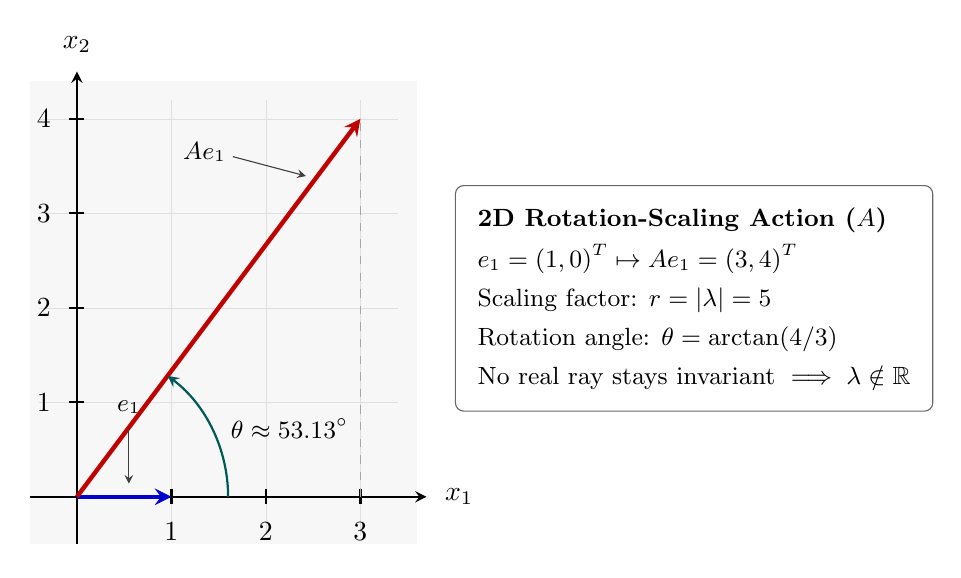
\begin{tikzpicture}[scale=1.2]
% Layer 1: Background fill
\fill[gray!6] (-0.5,-0.5) rectangle (3.6,4.4);

% Layer 2: Grid and Axes
\draw[gray!25, very thin] (-0.4,-0.4) grid (3.4,4.2);
\draw[->, >=stealth, thick] (-0.5,0) -- (3.7,0) node[right=3pt, black] {$x_1$};
\draw[->, >=stealth, thick] (0,-0.5) -- (0,4.5) node[above=3pt, black] {$x_2$};

% Microscopic tick marks
\draw[thick] (1,0.08) -- (1,-0.08) node[below=3pt, black] {$1$};
\draw[thick] (2,0.08) -- (2,-0.08) node[below=3pt, black] {$2$};
\draw[thick] (3,0.08) -- (3,-0.08) node[below=3pt, black] {$3$};
\draw[thick] (0.08,1) -- (-0.08,1) node[left=3pt, black] {$1$};
\draw[thick] (0.08,2) -- (-0.08,2) node[left=3pt, black] {$2$};
\draw[thick] (0.08,3) -- (-0.08,3) node[left=3pt, black] {$3$};
\draw[thick] (0.08,4) -- (-0.08,4) node[left=3pt, black] {$4$};

% Layer 3: Vectors, Auxiliary Lines, and Arcs
\draw[dashed, gray!70] (3,0) -- (3,4);
\draw[->, >=stealth, blue!80!black, ultra thick] (0,0) -- (1,0);
\draw[->, >=stealth, red!75!black, ultra thick] (0,0) -- (3,4);
\draw[->, >=stealth, teal!70!black, thick] (1.6,0) arc (0:53.13:1.6);

% Off-axis callouts
\draw[->, >=stealth, shorten >=2pt, black!75] (0.55,0.72) -- (0.55,0.08);
\draw[->, >=stealth, shorten >=2pt, black!75] (1.65,3.6) -- (2.48,3.38);

% Layer 4: Labels and Single-Node Legend
\node[black, font=\small] at (0.55,0.95) {$\displaystyle e_1$};
\node[black, font=\small] at (1.35,3.65) {$\displaystyle Ae_1$};
\node[black, font=\small] at (2.25,0.72) {$\displaystyle \theta \approx 53.13^\circ$};

\node[draw=black!60, fill=white, rounded corners=3pt, align=left, inner sep=8pt, anchor=west, text=black, font=\small] at (4.0,2.1) {
\textbf{2D Rotation-Scaling Action ($A$)}\\[4pt]
$\displaystyle e_1 = (1, 0)^T \mapsto Ae_1 = (3, 4)^T$\\[3pt]
Scaling factor: $\displaystyle r = |\lambda| = 5$\\[3pt]
Rotation angle: $\displaystyle \theta = \arctan(4/3)$\\[3pt]
No real ray stays invariant $\implies \lambda \notin \mathbb{R}$
};
\end{tikzpicture}
\end{center}

\noindent\rule{\textwidth}{0.4pt}

\noindent\textbf{Problem 23}

\textbf{Original Problem:} Find the characteristic polynomial, all complex eigenvalues, and one corresponding complex eigenvector for each eigenvalue of the matrix $A = \begin{bmatrix} 1 & -5 \\ 2 & -1 \end{bmatrix}$.

\textbf{Solution:} Compute $\operatorname{tr}(A) = 1 + (-1) = 0$ and $\det(A) = (1)(-1) - (-5)(2) = -1 + 10 = 9$. The characteristic polynomial is
\[
p(\lambda) = \lambda^2 - 0\lambda + 9 = \lambda^2 + 9 = 0 \implies \lambda_1 = 3i, \quad \lambda_2 = -3i.
\]
For $\lambda_1 = 3i$, solve $(A - 3iI)v = 0$:
\[
\begin{bmatrix} 1 - 3i & -5 \\ 2 & -1 - 3i \end{bmatrix}\begin{bmatrix} x_1 \\ x_2 \end{bmatrix} = \begin{bmatrix} 0 \\ 0 \end{bmatrix}.
\]
The second row gives $2x_1 + (-1 - 3i)x_2 = 0 \implies x_1 = \frac{1 + 3i}{2}x_2$ (which also satisfies Row 1 since $(1 - 3i)(1 + 3i) = 1 + 9 = 10 = 2(5)$). Choosing $x_2 = 2$ yields $v_1 = \begin{bmatrix} 1 + 3i \\ 2 \end{bmatrix}$. \\
For $\lambda_2 = -3i = \overline{\lambda_1}$, taking the complex conjugate of $v_1$ (since $A$ is real) gives $v_2 = \overline{v_1} = \begin{bmatrix} 1 - 3i \\ 2 \end{bmatrix}$.
\textit{Verification:} $Av_1 = \begin{bmatrix} 1 + 3i - 10 \\ 2 + 6i - 2 \end{bmatrix} = \begin{bmatrix} -9 + 3i \\ 6i \end{bmatrix} = 3i\begin{bmatrix} 1 + 3i \\ 2 \end{bmatrix}$, and similarly $Av_2 = -3i\,v_2$.

\noindent\rule{\textwidth}{0.4pt}

\noindent\textbf{Problem 24}

\textbf{Original Problem:} Find the characteristic polynomial (in factored and expanded forms) and all real and complex eigenvalues of the $3 \times 3$ matrix $A = \begin{bmatrix} 2 & 0 & 0 \\ 3 & -2 & -5 \\ 1 & 1 & 2 \end{bmatrix}$.

\textbf{Solution:} Expand $\det(A - \lambda I)$ along the first row (which contains two zeros):
\begin{align*}
p(\lambda) = \det\begin{bmatrix} 2 - \lambda & 0 & 0 \\ 3 & -2 - \lambda & -5 \\ 1 & 1 & 2 - \lambda \end{bmatrix} &= (2 - \lambda)\det\begin{bmatrix} -2 - \lambda & -5 \\ 1 & 2 - \lambda \end{bmatrix} \\
&= (2 - \lambda)\big[(-2 - \lambda)(2 - \lambda) - (-5)(1)\big] \\
&= (2 - \lambda)(\lambda^2 - 4 + 5) \\
&= (2 - \lambda)(\lambda^2 + 1).
\end{align*}
Expanding completely gives $p(\lambda) = -\lambda^3 + 2\lambda^2 - \lambda + 2$.
Setting $p(\lambda) = 0$ yields $2 - \lambda = 0$ or $\lambda^2 + 1 = 0$, so the eigenvalues are $\lambda_1 = 2$, $\lambda_2 = i$, and $\lambda_3 = -i$.
\textit{Verification:} $\operatorname{tr}(A) = 2 - 2 + 2 = 2 = 2 + i - i$, and $\det(A) = p(0) = 2 = 2 \cdot i \cdot (-i)$.

\noindent\rule{\textwidth}{0.4pt}

\noindent\textbf{Problem 25}

\textbf{Original Problem:} Consider the matrix $A = \begin{bmatrix} 5 & 2 & 0 \\ 0 & 5 & 0 \\ -1 & 3 & 2 \end{bmatrix}$. Find all eigenvalues of $A$, determine the algebraic multiplicity and geometric multiplicity of each eigenvalue by finding a basis for each eigenspace, and state whether $A$ is defective or diagonalizable.

\textbf{Solution:} Expand $\det(A - \lambda I)$ along the second row:
\[
p(\lambda) = \det\begin{bmatrix} 5 - \lambda & 2 & 0 \\ 0 & 5 - \lambda & 0 \\ -1 & 3 & 2 - \lambda \end{bmatrix} = (5 - \lambda)^2(2 - \lambda).
\]
Thus, $\lambda = 5$ has algebraic multiplicity $\operatorname{AM}(5) = 2$, and $\lambda = 2$ has algebraic multiplicity $\operatorname{AM}(2) = 1$.

For $\lambda = 2$, solve $(A - 2I)x = 0$:
\[
\begin{bmatrix} 3 & 2 & 0 \\ 0 & 3 & 0 \\ -1 & 3 & 0 \end{bmatrix}\begin{bmatrix} x_1 \\ x_2 \\ x_3 \end{bmatrix} = \begin{bmatrix} 0 \\ 0 \\ 0 \end{bmatrix} \implies x_2 = 0,\ x_1 = 0,\ x_3 \text{ free}.
\]
The eigenspace is $E_2 = \operatorname{span}\left\{\begin{bmatrix} 0 \\ 0 \\ 1 \end{bmatrix}\right\}$, so $\operatorname{GM}(2) = 1$.

For $\lambda = 5$, solve $(A - 5I)x = 0$:
\[
\begin{bmatrix} 0 & 2 & 0 \\ 0 & 0 & 0 \\ -1 & 3 & -3 \end{bmatrix}\begin{bmatrix} x_1 \\ x_2 \\ x_3 \end{bmatrix} = \begin{bmatrix} 0 \\ 0 \\ 0 \end{bmatrix}.
\]
Row 1 gives $2x_2 = 0 \implies x_2 = 0$. Substituting into Row 3 gives $-x_1 - 3x_3 = 0 \implies x_1 = -3x_3$, with $x_3$ free. Thus $E_5 = \operatorname{span}\left\{\begin{bmatrix} -3 \\ 0 \\ 1 \end{bmatrix}\right\}$, so $\operatorname{GM}(5) = 1$.
Because $\operatorname{GM}(5) = 1 < 2 = \operatorname{AM}(5)$, $A$ is \textbf{defective} and cannot be diagonalized.

\noindent\rule{\textwidth}{0.4pt}

\noindent\textbf{Problem 26}

\textbf{Original Problem:} Consider the two $3 \times 3$ matrices $A = \begin{bmatrix} 2 & 0 & 1 \\ 1 & 1 & -1 \\ 0 & 0 & 2 \end{bmatrix}$ and $B = \begin{bmatrix} 2 & 0 & 0 \\ 1 & 1 & -1 \\ 0 & 0 & 2 \end{bmatrix}$. (a) Show that $A$ and $B$ have the exact same characteristic polynomial and eigenvalues. (b) For the repeated eigenvalue $\lambda = 2$, compute the geometric multiplicity of $\lambda = 2$ in $A$ and in $B$. Which matrix is defective, which is diagonalizable, and can $A$ and $B$ be similar?

\textbf{Solution:}
\begin{enumerate}[label=(\alph*), topsep=3pt, itemsep=4pt]
    \item Expanding along Row 3 of $(A - \lambda I)$ and Row 1 of $(B - \lambda I)$ gives:
    \begin{align*}
    p_A(\lambda) &= (2 - \lambda)\det\begin{bmatrix} 2 - \lambda & 0 \\ 1 & 1 - \lambda \end{bmatrix} = (2 - \lambda)^2(1 - \lambda), \\
    p_B(\lambda) &= (2 - \lambda)\det\begin{bmatrix} 1 - \lambda & -1 \\ 0 & 2 - \lambda \end{bmatrix} = (2 - \lambda)^2(1 - \lambda).
    \end{align*}
    Both matrices share the exact same characteristic polynomial $(2 - \lambda)^2(1 - \lambda)$ and eigenvalues $\lambda = 2$ ($\operatorname{AM} = 2$) and $\lambda = 1$ ($\operatorname{AM} = 1$).
    \item For $A$ at $\lambda = 2$:
    \[
    A - 2I = \begin{bmatrix} 0 & 0 & 1 \\ 1 & -1 & -1 \\ 0 & 0 & 0 \end{bmatrix} \implies x_3 = 0 \text{ and } x_1 = x_2 \implies E_2(A) = \operatorname{span}\left\{\begin{bmatrix} 1 \\ 1 \\ 0 \end{bmatrix}\right\},
    \]
    so $\operatorname{GM}_A(2) = 1 < 2 = \operatorname{AM}_A(2)$. Hence $A$ is \textbf{defective}.

    For $B$ at $\lambda = 2$:
    \[
    B - 2I = \begin{bmatrix} 0 & 0 & 0 \\ 1 & -1 & -1 \\ 0 & 0 & 0 \end{bmatrix} \implies x_1 = x_2 + x_3 \quad (x_2, x_3 \text{ free}),
    \]
    so $E_2(B) = \operatorname{span}\left\{\begin{bmatrix} 1 \\ 1 \\ 0 \end{bmatrix}, \begin{bmatrix} 1 \\ 0 \\ 1 \end{bmatrix}\right\}$ and $\operatorname{GM}_B(2) = 2 = \operatorname{AM}_B(2)$. Since $\lambda = 1$ also has $\operatorname{GM}_B(1) = 1 = \operatorname{AM}_B(1)$, $B$ has $3$ linearly independent eigenvectors and is \textbf{diagonalizable} (non-defective).
    Because similar matrices preserve eigenspace dimensions (and diagonalizability), $A$ and $B$ \textbf{cannot be similar} despite sharing the same characteristic polynomial.
\end{enumerate}

\noindent\rule{\textwidth}{0.4pt}

\noindent\textbf{Problem 27}

\textbf{Original Problem:} Consider the parameterized matrix $A_c = \begin{bmatrix} 3 & c & 1 \\ 0 & 3 & 0 \\ 0 & 2 & -1 \end{bmatrix}$, $c \in \mathbb{R}$. (a) Find the characteristic polynomial and eigenvalues of $A_c$, noting whether they depend on $c$. (b) Find the algebraic and geometric multiplicities of each eigenvalue as a function of $c$. For which value(s) of $c$ is $A_c$ diagonalizable (non-defective), and for which value(s) is it defective?

\textbf{Solution:}
\begin{enumerate}[label=(\alph*), topsep=3pt, itemsep=4pt]
    \item Expanding $\det(A_c - \lambda I)$ down the first column gives:
    \[
    p(\lambda) = (3 - \lambda)\det\begin{bmatrix} 3 - \lambda & 0 \\ 2 & -1 - \lambda \end{bmatrix} = (3 - \lambda)^2(-1 - \lambda) = -(\lambda - 3)^2(\lambda + 1).
    \]
    Neither the characteristic polynomial nor the eigenvalues $\lambda = 3$ ($\operatorname{AM} = 2$) and $\lambda = -1$ ($\operatorname{AM} = 1$) depend on $c$.
    \item For $\lambda = -1$, since $1 \le \operatorname{GM}(-1) \le \operatorname{AM}(-1) = 1$, we always have $\operatorname{GM}(-1) = 1$ for every $c \in \mathbb{R}$. For $\lambda = 3$, solve $(A_c - 3I)x = 0$:
    \[
    \begin{bmatrix} 0 & c & 1 \\ 0 & 0 & 0 \\ 0 & 2 & -4 \end{bmatrix}\begin{bmatrix} x_1 \\ x_2 \\ x_3 \end{bmatrix} = \begin{bmatrix} 0 \\ 0 \\ 0 \end{bmatrix}.
    \]
    Row 3 gives $2x_2 - 4x_3 = 0 \implies x_2 = 2x_3$. Substituting into Row 1 yields $c(2x_3) + x_3 = (2c + 1)x_3 = 0$.
    \begin{itemize}[topsep=2pt, itemsep=2pt]
        \item \textit{Case 1 ($c = -\frac{1}{2}$):} Then $2c + 1 = 0$, so $(2c + 1)x_3 = 0$ holds identically. Both $x_1$ and $x_3$ are free variables, yielding two linearly independent eigenvectors $\begin{bmatrix} 1 \\ 0 \\ 0 \end{bmatrix}$ and $\begin{bmatrix} 0 \\ 2 \\ 1 \end{bmatrix}$. Thus $\operatorname{GM}(3) = 2 = \operatorname{AM}(3)$, and $A_c$ is \textbf{diagonalizable}.
        \item \textit{Case 2 ($c \neq -\frac{1}{2}$):} Then $2c + 1 \neq 0$ forces $x_3 = 0$ and $x_2 = 0$, leaving only $x_1$ free. Thus $\operatorname{GM}(3) = 1 < 2 = \operatorname{AM}(3)$, so $A_c$ is \textbf{defective}.
    \end{itemize}
\end{enumerate}

\subsection{Solutions to Real-World Modeling: PCA and Markov Chains (Problems 28--30)}

\noindent\textbf{Problem 28}

\textbf{Original Problem:} In quantitative finance, the sample covariance matrix of daily returns (in $\%^2$) for two correlated technology equities is $\Sigma = \begin{bmatrix} 5 & 2 \\ 2 & 2 \end{bmatrix}$. (a) Find the characteristic polynomial and eigenvalues $\lambda_1 \ge \lambda_2$ of $\Sigma$, verifying that both are real and non-negative. (b) Compute the total variance $\operatorname{tr}(\Sigma)$ and determine the exact fraction (and percentage) of total variance explained by the first principal component. (c) Find a unit eigenvector $v_1$ corresponding to $\lambda_1$ (the first principal component loading vector).

\textbf{Solution:}
\begin{enumerate}[label=(\alph*), topsep=3pt, itemsep=4pt]
    \item Using $\operatorname{tr}(\Sigma) = 5 + 2 = 7$ and $\det(\Sigma) = (5)(2) - (2)(2) = 6$:
    \[
    p(\lambda) = \lambda^2 - 7\lambda + 6 = (\lambda - 6)(\lambda - 1) = 0 \implies \lambda_1 = 6, \quad \lambda_2 = 1.
    \]
    Both eigenvalues are real and non-negative ($6 \ge 1 \ge 0$), as guaranteed by the Spectral Theorem for symmetric positive semi-definite covariance matrices.
    \item Total variance is $\operatorname{tr}(\Sigma) = 5 + 2 = 7 = \lambda_1 + \lambda_2$. The fraction of variance captured by the first principal component is
    \[
    \frac{\lambda_1}{\lambda_1 + \lambda_2} = \frac{6}{7} \approx 85.71\%.
    \]
    \item For $\lambda_1 = 6$, solve $(\Sigma - 6I)x = 0$:
    \[
    \begin{bmatrix} -1 & 2 \\ 2 & -4 \end{bmatrix}\begin{bmatrix} x_1 \\ x_2 \end{bmatrix} = \begin{bmatrix} 0 \\ 0 \end{bmatrix} \implies x_1 = 2x_2.
    \]
    Taking $x = \begin{bmatrix} 2 \\ 1 \end{bmatrix}$ gives $\|x\| = \sqrt{2^2 + 1^2} = \sqrt{5}$, so the unit loading vector is
    \[
    v_1 = \frac{1}{\sqrt{5}}\begin{bmatrix} 2 \\ 1 \end{bmatrix}.
    \]
\end{enumerate}

\noindent\rule{\textwidth}{0.4pt}

\noindent\textbf{Problem 29}

\textbf{Original Problem:} An algorithmic trading model uses a $3$-factor centered covariance matrix $\Sigma = \begin{bmatrix} 6 & 0 & 4 \\ 0 & 4 & 0 \\ 4 & 0 & 6 \end{bmatrix}$. (a) Find all eigenvalues $\lambda_1 \ge \lambda_2 \ge \lambda_3$ of $\Sigma$ by strategically expanding $\det(\Sigma - \lambda I) = 0$. (b) Verify your eigenvalues using $\operatorname{tr}(\Sigma)$ and $\det(\Sigma)$. (c) If the model projects the feature space onto the top $k$ principal components needed to capture at least $80\%$ of total variance, find the minimum required dimension $k$ and the exact percentage of variance captured.

\textbf{Solution:}
\begin{enumerate}[label=(\alph*), topsep=3pt, itemsep=4pt]
    \item Expanding $\det(\Sigma - \lambda I)$ along the second row (two zeros):
    \begin{align*}
    p(\lambda) = \det\begin{bmatrix} 6 - \lambda & 0 & 4 \\ 0 & 4 - \lambda & 0 \\ 4 & 0 & 6 - \lambda \end{bmatrix} &= (4 - \lambda)\big[(6 - \lambda)^2 - 16\big] \\
    &= (4 - \lambda)(6 - \lambda - 4)(6 - \lambda + 4) \\
    &= (4 - \lambda)(2 - \lambda)(10 - \lambda).
    \end{align*}
    Ordering from largest to smallest gives $\lambda_1 = 10$, $\lambda_2 = 4$, and $\lambda_3 = 2$.
    \item $\operatorname{tr}(\Sigma) = 6 + 4 + 6 = 16 = 10 + 4 + 2$, and $\det(\Sigma) = 4(36 - 16) = 80 = 10 \cdot 4 \cdot 2$. Both identities check out.
    \item Total variance is $16$. Checking cumulative variance ratios:
    \begin{align*}
    k = 1: \quad \frac{\lambda_1}{16} &= \frac{10}{16} = 62.5\% < 80\%, \\
    k = 2: \quad \frac{\lambda_1 + \lambda_2}{16} &= \frac{10 + 4}{16} = \frac{14}{16} = \frac{7}{8} = 87.5\% \ge 80\%.
    \end{align*}
    Thus, the minimum required dimension is $k = 2$, capturing $87.5\%$ of total variance.
\end{enumerate}

\noindent\rule{\textwidth}{0.4pt}

\noindent\textbf{Problem 30}

\textbf{Original Problem:} A quantitative analyst models daily transitions between two market regimes—Bull (State $1$) and Bear (State $2$)—using the column-stochastic transition matrix $T = \begin{bmatrix} 0.8 & 0.3 \\ 0.2 & 0.7 \end{bmatrix}$, where $T_{ij}$ denotes the probability of moving from regime $j$ today to regime $i$ tomorrow. (a) Find the characteristic polynomial and all eigenvalues of $T$, and explain why $\lambda = 1$ must be an eigenvalue of any column-stochastic matrix. (b) Find the steady-state probability vector $\pi = \begin{bmatrix} \pi_1 \\ \pi_2 \end{bmatrix}$ (an eigenvector for $\lambda = 1$ with non-negative entries summing to $1$). (c) Express the initial state $x_0 = \begin{bmatrix} 1 \\ 0 \end{bmatrix}$ as a linear combination of eigenvectors of $T$, and evaluate $\lim_{k \to \infty} T^k x_0$.

\textbf{Solution:}
\begin{enumerate}[label=(\alph*), topsep=3pt, itemsep=4pt]
    \item Here $\operatorname{tr}(T) = 0.8 + 0.7 = 1.5$ and $\det(T) = (0.8)(0.7) - (0.3)(0.2) = 0.56 - 0.06 = 0.5$. Thus
    \[
    p(\lambda) = \lambda^2 - 1.5\lambda + 0.5 = (\lambda - 1)(\lambda - 0.5) = 0 \implies \lambda_1 = 1, \quad \lambda_2 = 0.5.
    \]
    For any column-stochastic matrix $T$, each column sums to $1$, so each row of $T^T$ sums to $1$; hence $T^T \mathbf{1} = 1 \cdot \mathbf{1}$ where $\mathbf{1}$ is the all-ones vector. Thus $1$ is an eigenvalue of $T^T$, and since $T$ and $T^T$ share the same eigenvalues (Problem 17), $\lambda = 1$ must be an eigenvalue of $T$.
    \item Solve $(T - I)\pi = 0$:
    \[
    \begin{bmatrix} -0.2 & 0.3 \\ 0.2 & -0.3 \end{bmatrix}\begin{bmatrix} \pi_1 \\ \pi_2 \end{bmatrix} = \begin{bmatrix} 0 \\ 0 \end{bmatrix} \implies 0.2\pi_1 = 0.3\pi_2 \implies \pi_1 = \frac{3}{2}\pi_2.
    \]
    Imposing $\pi_1 + \pi_2 = 1$ gives $\frac{5}{2}\pi_2 = 1 \implies \pi_2 = 0.4$ and $\pi_1 = 0.6$, so $\pi = \begin{bmatrix} 0.6 \\ 0.4 \end{bmatrix}$.
    \item For $\lambda_2 = 0.5$, $(T - 0.5I)v = \begin{bmatrix} 0.3 & 0.3 \\ 0.2 & 0.2 \end{bmatrix}v = 0$ gives eigenvector $v_2 = \begin{bmatrix} 1 \\ -1 \end{bmatrix}$. Solving $x_0 = c_1 \pi + c_2 v_2$:
    \[
    \begin{bmatrix} 1 \\ 0 \end{bmatrix} = c_1\begin{bmatrix} 0.6 \\ 0.4 \end{bmatrix} + c_2\begin{bmatrix} 1 \\ -1 \end{bmatrix}.
    \]
    Adding both components gives $1 = c_1(0.6 + 0.4) = c_1$, and the second component gives $0 = 0.4 - c_2 \implies c_2 = 0.4$. Therefore,
    \[
    T^k x_0 = 1^k \pi + 0.4(0.5)^k v_2 = \begin{bmatrix} 0.6 \\ 0.4 \end{bmatrix} + 0.4(0.5)^k\begin{bmatrix} 1 \\ -1 \end{bmatrix}.
    \]
    Since $\lim_{k \to \infty} (0.5)^k = 0$, we obtain $\lim_{k \to \infty} T^k x_0 = \pi = \begin{bmatrix} 0.6 \\ 0.4 \end{bmatrix}$.
\end{enumerate}

\subsection{Solutions to Diagnostic Testing: Find the Flaw (Problems 31--34)}

\noindent\textbf{Problem 31}

\textbf{Original Problem:} \textit{Find the Flaw:} Below is a student's attempt to find the characteristic polynomial and eigenvalues of $A = \begin{bmatrix} 5 & 4 \\ 1 & 2 \end{bmatrix}$: ``Using the $2 \times 2$ shortcut formula, $p(\lambda) = \lambda^2 + \operatorname{tr}(A)\lambda + \det(A) = \lambda^2 + 7\lambda + 6 = (\lambda + 6)(\lambda + 1) = 0$, yielding eigenvalues $\lambda_1 = -6$ and $\lambda_2 = -1$.'' Identify the flaw, explain why it is wrong in one clear sentence, and provide the correct characteristic polynomial and eigenvalues.

\textbf{Solution:}
\begin{itemize}[topsep=3pt, itemsep=3pt]
    \item \textbf{Flaw Identification and Explanation:} The student used $+\operatorname{tr}(A)\lambda$ instead of $-\operatorname{tr}(A)\lambda$ in the $2 \times 2$ characteristic polynomial formula, because expanding $(a_{11} - \lambda)(a_{22} - \lambda) - a_{12}a_{21}$ produces $\lambda^2 - (a_{11} + a_{22})\lambda + \det(A)$.
    \item \textbf{Correct Solution:} With $\operatorname{tr}(A) = 7$ and $\det(A) = 6$, the correct characteristic polynomial is
    \[
    p(\lambda) = \lambda^2 - 7\lambda + 6 = (\lambda - 6)(\lambda - 1) = 0,
    \]
    so the eigenvalues are $\lambda_1 = 6$ and $\lambda_2 = 1$.
\end{itemize}

\noindent\rule{\textwidth}{0.4pt}

\noindent\textbf{Problem 32}

\textbf{Original Problem:} \textit{Find the Flaw:} Below is a student's attempt to find the characteristic polynomial and eigenvalues of $A = \begin{bmatrix} 2 & -1 & 4 \\ 0 & 5 & 3 \\ 0 & 0 & -3 \end{bmatrix}$: ``Expanding $\det\begin{bmatrix} 2 - \lambda & -1 & 4 \\ 0 & 5 & 3 \\ 0 & 0 & -3 \end{bmatrix}$ along the first column gives $(2 - \lambda)[(5)(-3) - 0] = 15\lambda - 30$, so the only eigenvalue is $\lambda = 2$.'' Identify the flaw, explain why it is wrong in one clear sentence, and provide the correct characteristic polynomial (factored and expanded) and all eigenvalues.

\textbf{Solution:}
\begin{itemize}[topsep=3pt, itemsep=3pt]
    \item \textbf{Flaw Identification and Explanation:} The student subtracted $\lambda$ only from the $(1, 1)$ entry instead of every main diagonal entry, failing to construct the matrix $A - \lambda I$ properly.
    \item \textbf{Correct Solution:} Because $A - \lambda I = \begin{bmatrix} 2 - \lambda & -1 & 4 \\ 0 & 5 - \lambda & 3 \\ 0 & 0 & -3 - \lambda \end{bmatrix}$ is upper triangular, its characteristic polynomial is the product of all diagonal entries:
    \[
    p(\lambda) = (2 - \lambda)(5 - \lambda)(-3 - \lambda) = -\lambda^3 + 4\lambda^2 + 11\lambda - 30.
    \]
    Setting $p(\lambda) = 0$ gives eigenvalues $\lambda = 2, 5, -3$ (each with algebraic multiplicity $1$).
\end{itemize}

\noindent\rule{\textwidth}{0.4pt}

\noindent\textbf{Problem 33}

\textbf{Original Problem:} \textit{Find the Flaw:} For $A = \begin{bmatrix} 2 & 3 \\ 1 & 4 \end{bmatrix}$, a student correctly finds eigenvalues $5$ and $1$, and then writes: ``To find the eigenvalues of $A^3$, we multiply each eigenvalue of $A$ by $3$, giving eigenvalues $15$ and $3$.'' Identify the flaw, explain why it is wrong in one clear sentence, and provide the correct eigenvalues of $A^3$ (along with a trace/determinant verification).

\textbf{Solution:}
\begin{itemize}[topsep=3pt, itemsep=3pt]
    \item \textbf{Flaw Identification and Explanation:} If $Ax = \lambda x$ with $x \neq 0$, repeated multiplication by $A$ gives $A^3 x = \lambda^3 x$, so the eigenvalues of $A^3$ are the cubes $\lambda^3$ rather than the scalar multiples $3\lambda$.
    \item \textbf{Correct Solution:} Since the eigenvalues of $A$ are $5$ and $1$, the eigenvalues of $A^3$ are $5^3 = 125$ and $1^3 = 1$.
    \textit{Verification:} Direct multiplication yields $A^2 = \begin{bmatrix} 7 & 18 \\ 6 & 19 \end{bmatrix}$ and $A^3 = \begin{bmatrix} 32 & 93 \\ 31 & 94 \end{bmatrix}$, confirming $\operatorname{tr}(A^3) = 32 + 94 = 126 = 125 + 1$ and $\det(A^3) = (32)(94) - (93)(31) = 3008 - 2883 = 125 = 125 \cdot 1$.
\end{itemize}

\noindent\rule{\textwidth}{0.4pt}

\noindent\textbf{Problem 34}

\textbf{Original Problem:} \textit{Find the Flaw:} A $3 \times 3$ matrix $A$ has characteristic polynomial $p(\lambda) = -\lambda^3 + 8\lambda^2 - 16\lambda = -\lambda(\lambda - 4)^2$. A student writes: ``Because $\lambda = 4$ is a nonzero eigenvalue with algebraic multiplicity $2$ (accounting for the majority of the eigenvalues), the matrix stretches vectors along those directions, so $A$ is invertible.'' Identify the flaw, explain why it is wrong in one clear sentence, and provide the correct conclusion supported by $\det(A)$ and the Invertible Matrix Theorem.

\textbf{Solution:}
\begin{itemize}[topsep=3pt, itemsep=3pt]
    \item \textbf{Flaw Identification and Explanation:} A matrix is invertible if and only if \textit{none} of its eigenvalues equals $0$, so the presence of $\lambda = 0$ as a root forces $\det(A) = 0$ regardless of how many nonzero eigenvalues or high-multiplicity roots exist.
    \item \textbf{Correct Solution:} Because $\lambda = 0$ is an eigenvalue, $\det(A) = p(0) = 0 \cdot 4 \cdot 4 = 0$ and the equation $Ax = 0$ possesses a nontrivial solution $x \neq 0$; by the Invertible Matrix Theorem, $A$ is \textbf{not invertible} (singular).
\end{itemize}

\newpage

\section{Concept Checklist and Question Mapping Reference Index}

\renewcommand{\arraystretch}{1.5}
\begin{tabularx}{\textwidth}{l X >{$\displaystyle}l<{$} p{1.2in}}
\toprule
\textbf{ID} & \textbf{Concept and Problem Type} & \multicolumn{1}{l}{\textbf{Key Formula / Identity}} & \textbf{Questions} \\
\midrule
C1 & Basic $2 \times 2$ Characteristic Polynomials \& Distinct Real Eigenvalues & \lambda^2 - \operatorname{tr}(A)\lambda + \det(A) = 0 & 1, 2, 19, 20, 28, 30, 31, 33 \\
\addlinespace[4pt]
C2 & Repeated Eigenvalues, Parameter Tuning, \& Algebraic Multiplicity & (\lambda - \lambda_0)^m = 0 \quad (m \ge 2) & 3, 4, 5, 8, 9, 10, 25, 26, 27 \\
\addlinespace[4pt]
C3 & Strategic $3 \times 3$ Expansion (Zero-Rich Lines, Pre-Factored Forms, Rational Roots) & \det(A - \lambda I) = \sum \pm (a_{ij} - \lambda\delta_{ij}) C_{ij} & 5, 6, 7, 8, 9, 24, 29 \\
\addlinespace[4pt]
C4 & Upper/Lower Triangular \& Block-Triangular Eigenvalue Properties & \det(A - \lambda I) = \prod_{i=1}^{n} (a_{ii} - \lambda) & 10, 11, 25, 26, 27, 32 \\
\addlinespace[4pt]
C5 & Trace/Determinant Identities \& Scalar-Substitution ($\lambda = 0$, $\lambda = c$) Tricks & \operatorname{tr}(A) = \sum_{i=1}^{n} \lambda_i,\ \ \det(A) = \prod_{i=1}^{n} \lambda_i & 4, 12, 13, 14, 29 \\
\addlinespace[4pt]
C6 & Invertibility, Zero Eigenvalues, Null Spaces, \& Conceptual True/False & Ax = 0,\ x \neq 0 \iff \det(A) = 0 & 14, 15, 16, 17, 34 \\
\addlinespace[4pt]
C7 & Similarity Transformations, Matrix Powers $A^k$, Diagonalization, \& Polynomials $q(A)$ & \det(PAP^{-1} - \lambda I) = \det(A - \lambda I) & 18, 19, 20, 21, 33 \\
\addlinespace[4pt]
C8 & Complex Conjugate Eigenvalues \& Rotational/Oscillatory Geometry & \lambda = \alpha \pm \beta i \quad (\Delta < 0) & 22, 23, 24 \\
\addlinespace[4pt]
C9 & Geometric vs.\ Algebraic Multiplicity, Eigenspaces, \& Defective Matrices & 1 \le \operatorname{GM}(\lambda) \le \operatorname{AM}(\lambda) & 25, 26, 27 \\
\addlinespace[4pt]
C10 & Applied Modeling: PCA Covariance Variance Capture \& Markov Steady States & \Sigma v = \lambda v,\ \ T\pi = 1 \cdot \pi & 28, 29, 30 \\
\addlinespace[4pt]
C11 & Diagnostic Error Analysis (``Find the Flaw''): Signs, Diagonals, Powers, \& $0$-Roots & A^k x = \lambda^k x,\ \ (A - \lambda I) & 31, 32, 33, 34 \\
\bottomrule
\end{tabularx}

\end{document}